\documentclass{optica-article}

\journal{opticajournal} % for journals or Optica Open

\articletype{Research Article}

\usepackage{lineno}
\usepackage{textcomp}
\usepackage{placeins}
\usepackage{graphicx}
\usepackage{float}
\usepackage{subcaption}

\linenumbers % Turn off line numbering for Optica Open preprint submissions.

\begin{document}

\title{Characterising measurements of vessel diameter in optical coherence tomography angiography and correcting artefact induced underestimation}

\author{Yash Patel,\authormark{1} Prajakta Belekar,\authormark{1} Georg Ladurner,\authormark{1} Sybren Worm,\authormark{1} Lucas May,\authormark{1} Maria Varaka,\authormark{1} Theresa Rohrmoser,\authormark{1} Fernando Garc\'{i}a-Ram\'{i}rez,\authormark{1} Ren\'{e} Werkmeister,\authormark{1} Bernhard Baumann,\authormark{1,2} and Conrad W. Merkle\authormark{1,*}}

\address{\authormark{1}Center for Medical Physics and Biomedical Engineering, Medical University of Vienna, Währinger Gürtel 18-20/4L, 1090 Vienna, Austria\\
\authormark{2}Institute of Biomedical Physics, Medical University of Innsbruck, Müllerstraße 44, 6020 Innsbruck, Austria}

\email{\authormark{*}conrad.merkle@meduniwien.ac.at} %% email address is required; see note below about the corresponding author designation

% \section{Corresponding author}

% We require manuscripts to identify only a single corresponding author. The corresponding author typically is the person who submits the manuscript and handles correspondence throughout the peer review and publication process. Alternatively, you may choose not to identify a corresponding author and instead use an author note to indicate equal author contributions. Only the corresponding author will have an asterisk attached to their e-mail address. Additional co-author e-mail addresses will have a superscript number in the numerical order of the affiliations. 

% \begin{verbatim}
% \author{Author One\authormark{1} and 
% Author Two\authormark{2,*}}

% \address{\authormark{1}Peer Review, Publications Department,
% Optica Publishing Group, 2010 Massachusetts Avenue NW,
% Washington, DC 20036, USA\\
% \authormark{2}Publications Department, Optica Publishing Group,
% 2010 Massachusetts Avenue NW, Washington, DC 20036, USA\\

% \email{\authormark{*}xyz@optica.org}
% \end{verbatim}

% This format will generate the following appearance:  

% \bigskip

% \author{Author One\authormark{1} and Author Two\authormark{2,*}}

% \address{\authormark{1}Peer Review, Publications Department,
% Optica Publishing Group, 2010 Massachusetts Avenue NW,
% Washington, DC 20036, USA\\
% \authormark{2}Publications Department, Optica Publishing Group,
% 2010 Massachusetts Avenue NW, Washington, DC 20036, USA\\
% %\authormark{3}xyz@optica.org}

% \email{\authormark{*}xyz@optica.org}}

% \medskip

% If other statements about author contribution and contact are needed, they can be added in addition to the corresponding author designation.
% \begin{verbatim}
% \author{Author One\authormark{1,$\dag$} and 
% Author Two\authormark{2,$\dag$,*}}

% \address{\authormark{1}Peer Review, Publications Department,
% Optica Publishing Group, 2010 Massachusetts Avenue NW,
% Washington, DC 20036, USA\\
% \authormark{2}Publications Department, Optica Publishing Group,
% 2010 Massachusetts Avenue NW, Washington, DC 20036, USA\\
% \authormark{$\dag$}The authors contributed equally to
% this work.\\
% \authormark{*}xyz@optica.org}}
% \end{verbatim}

% This format will generate the following appearance:

% \medskip

% \author{Author One\authormark{1,\dag} and Author Two\authormark{2,\dag,*}}

% \address{\authormark{1}Peer Review, Publications Department,
% Optica Publishing Group, 2010 Massachusetts Avenue NW, Washington, DC 20036, USA\\
% \authormark{2}Publications Department, Optica Publishing Group, 2010 Massachusetts Avenue NW, Washington, DC 20036, USA\\
% \authormark{\dag}The authors contributed equally to this work.\\
% \authormark{*}xyz@optica.org}
% \medskip

% use {asbstract*} to suppress the copyright line. Copyright information will be added in production

\begin{abstract*} 
% Abstract

% ~166 words:
Vessel diameter is a widely used biomarker of vascular health, commonly assessed in the retina using optical coherence tomography angiography (OCTA). However, shear-induced alignment of red blood cells at vessel edges reduces backscattering and suppresses the OCTA signal. This leads to systematic underestimation of vessel diameter. In this study, we established ground-truth diameters in the in vivo mouse retina using Intralipid contrast enhancement, compared binary mask based calculation against model-based profile fitting on maximum and mean intensity projections, and used flicker stimulation to evaluate the performance of each method. Before contrast, a generalised Gaussian fit to the maximum intensity projection retained the strongest linear relationship with ground truth of all methods tested, although it underestimated diameter by approximately 35\%, making it correctable by calibration. Post-contrast, the same fit applied to the mean intensity projection agreed with ground truth ($m = 1.001$, $R^2 = 0.97$). Under flicker stimulation, model-based fitting detected the expected vasodilation, whereas binary mask based calculation instead reported vasoconstriction. These findings characterise OCTA diameter underestimation and establish model-based fitting as a practical means of correcting it.

\end{abstract*}

%%%%%%%%%%%%%%%%%%%%%%%%%%  body  %%%%%%%%%%%%%%%%%%%%%%%%%%
\section{Introduction}
% Introduction

Vessel diameter is an important biomarker that can provide valuable information regarding local vascular health. Thickening of the arteriolar wall has been shown to narrow the vessel lumen in proliferative diabetic retinopathy~\cite{uenoAssociationChangesRetinal2021}. Retinal arteriolar narrowing has been shown to precede and predict the onset of systemic hypertension~\cite{ikramRetinalVesselDiameters2006}. In glaucoma suspects, reduced vessel diameter has been shown to track both retinal ganglion cell dysfunction and visual field loss~\cite{tirsiRetinalVesselDiameter2025}. Diameter changes are also informative beyond the eye, where a meta-analysis of observational studies found smaller retinal arteriolar caliber to be associated with coronary heart disease~\cite{liangRetinalVascularCaliber2022}. Different diseases have been shown to preferentially affect different plexuses, with glaucoma altering the superficial vascular complex~\cite{takusagawaProjectionResolvedOptical2017} while diabetic retinopathy~\cite{hwangVisualization3Distinct2016} and retinal vein occlusion~\cite{coscasOpticalCoherenceTomography2016} affect the deeper plexuses more severely. Combined with measurements of blood flow, diameter can also be used to investigate local blood pressure and vessel elasticity~\cite{kannenkerilRetinalVascularResistance2018,mynardMeasurementAnalysisInterpretation2020,seabraSilicoBloodPressure2022}. For these reasons, it is imperative that accurate measurements of vessel diameter be used for these extrapolations or when modeling behaviours of flow in digital twins~\cite{hernandezLinkingVascularStructure2024,hernandezMicrovascularRetinalDigital2026}. Optical imaging techniques are often used to measure vessel diameter due to their high resolution, but accurate measurement of vessel size is more difficult than it first appears.

Optical coherence tomography (OCT) is a non-invasive optical imaging method, which uses interferometry to measure the transit time of light that is backscattered from a sample, thereby producing depth-resolved images of tissue~\cite{huangOpticalCoherenceTomography1991,fercherVivoOpticalCoherence1993}. Optical coherence tomography angiography (OCTA) is an extension of OCT that visualizes vascular perfusion using the motion contrast from red blood cells (RBCs)~\cite{makitaOpticalCoherenceAngiography2006,srinivasanRapidVolumetricAngiography2010,taoSinglepassVolumetricBidirectional2008,wangThreeDimensionalOptical2007}. Over the years, OCTA has demonstrated widespread acceptance and use for clinical evaluations of vascular features in relation to disease~\cite{javedOpticalCoherenceTomography2023}. OCT angiograms can be used to evaluate characteristics on the scale of vascular layers by measuring vascular density or non-perfusion zones~\cite{tanApproachesQuantifyOptical2020,hwangVisualization3Distinct2016,coscasOpticalCoherenceTomography2016,takusagawaProjectionResolvedOptical2017,zabelComparisonRetinalMicrovasculature2019,tanApplicationOpticalCoherence2021}, or it can be used to guage vessel size~\cite{yaoComparisonRetinalVessel2021} or tortuosity~\cite{leeQUANTIFICATIONRETINALVESSEL2018}.

Analysis of OCTA datasets is typically achieved by performing a maximum intensity projection of a 3D vascular network to compress it into 2D before binarising the resulting angiogram using a global or local binarisation method. From this binarised angiogram, various vascular metrics can then be quantified. Importantly, there are many methods for performing this binarisation step and the choice of method can significantly affect the reported vascular metrics, with no clear consensus for a one size fits all approach~\cite{mehtaImpactBinarizationThresholding2019,rabioloComparisonMethodsQuantify2018,borrelliOPTICALCOHERENCETOMOGRAPHY2021,freedmanImpactImageProcessing2022,arrigoImpactDifferentThresholds2021}. Similarly, there are vascular enhancement algorithms to highlight structures that resemble vessels before quantification, but these methods also risk affecting the apparent size of the vessels in the network~\cite{freedmanImpactImageProcessing2022,hongIntrasessionRepeatabilityQuantitative2020,hongEffectVesselEnhancement2020}.

Furthermore, OCT is prone to certain artifacts which specifically affect visualization of the vasculature~\cite{cimallaShearFlowinducedOptical2011,zhuVisibilityMicrovesselsOptical2020,bernucciInvestigationArtifactsRetinal2018}. When viewed in cross-section, large vessels often demonstrate an hourglass appearance with stronger scattering in the center than at the sides. This appearance is due to orientation effects of RBCs, which align with the blood flow, causing a reduced scattering cross-section at the sides of the vessels~\cite{cimallaShearFlowinducedOptical2011}. We hypothesise that these artifacts may lead to underestimations of measurements of vessel diameter. To compensate for these artifacts, OCT contrast agents such as Intralipid have previously been used to increase intravascular intensity signals, particularly in regions where RBC scattering is diminished~\cite{panUltrasensitiveDetection3D2014,merkleDynamicContrastOptical2016,merkleLaminarMicrovascularTransit2016,zhuVisibilityMicrovesselsOptical2020,bernucciInvestigationArtifactsRetinal2018}.  

In this study we examine different methods of measuring vessel diameter from in vivo OCT scans of mouse retinal vasculature, and we use a contrast agent to obtain ground truth vessel diameter measurements for comparison. In addition to traditional binarisation-based methods, we also employ model-based methods for quantifying vessel diameter. Traditional Gaussian models have been employed for vessel diameter measurements in techniques such as fluorescein angiography~\cite{zhouDetectionQuantificationRetinopathy1994} and fundus photography~\cite{lowellMeasurementRetinalVessel2004} (based on other optical imaging methods) and OCT~\cite{leahyMapping3DConnectivity2015}, but we expand this by also investigating the generalized Gaussian model. As part of this study, we measure how much diameter is underestimated from enface projections and evaluate how reliably it can be compensated through calibration. Flicker stimulation is well established to evoke vasodilation in the retina~\cite{garhoferDiffuseLuminanceFlicker2004,sharifizadFactorsDeterminingFlickerinduced2016,michelsonFlickeringLightIncreases2002,aschingerEffectofDiffuse2017,kornfieldRegulationBloodFlow2014,shihQuantitativeRetinalChoroidal2013,sonOpticalCoherenceTomography2016}. After identifying the best methods for quantifying diameter and compensating for underestimations, we finally evaluated a test scenario using flicker stimulation to induce a measurable change in diameter to evaluate the performance of different methods.

%\section{Introduction}

% General structure of intro:
% Why diameter is an important measurment
% Brief OCTA Introduction
% Difficulty of OCTA quantification (different methods yield different results)
% Artefact contributions and diameter underestimation
% Proposed solution that we investigate here and evaluation of different methods in a test scenario (vessel dilation)

% https://www.nature.com/articles/s41598-021-84067-2
% https://qims.amegroups.org/article/view/51210/html
% https://jamanetwork.com/journals/jamaophthalmology/fullarticle/415121
% https://www.sciencedirect.com/science/article/pii/S0307904X23002913
% https://www.pnas.org/doi/10.1073/pnas.2521872123

%In addition to thresholding-based variability, we hypothesize that OCTA metrics are also affected by OCT artifacts caused by the non-uniform backscattering profiles of red blood cells (RBCs).  Because RBCs have a distinct bi-concave disc shape, they more effectively backscatter light when aligned perpendicular to the beam, rather than parallel to it.  It has already been observed that in large vessels, a so-called hourglass artifact appears when viewed cross-sectionally.  This is caused by the alignment of the RBCs with the vessel walls while under laminar flow, where the RBCs are perpendicular to the beam in the center of the vessels and parallel to the beam at the edges of the vessels.  This artifact artificially suppresses the OCT and OCTA signals at the edges of the vessels, making them appear more narrow when projected into an en-face view, which is the preferred way of displaying angiographic data.  Here we use contrast enhanced OCT (CE-OCT) to investigate how significant these effects are and how they can be corrected.

%Optical coherence tomography (OCT) is a non-invasive optical imaging method, which uses interferometry to measure the transit time of light that is backscattered from a sample.  OCT has found widespread clinical use in ophthalmology with XXX number of systems and XXX OCT scans performed annually around the world.  OCT angiography (OCTA) is a functional extension of OCT which highlights motion between repeated OCT scans to generate images of vascular networks.  Typically, OCTA signals are first calculated from the OCT intensity and/or phase information, segmented in 3D manually, algorithmically, or using a deep learning approach, and finally compressed into a 2D image using a maximum intensity projection.  These 2D vascular maps can then be binarised by using a global or adaptive threshold, and finally vascular metrics such as vessel density and diameter can be computed.  Of these processing stages, the thresholding step is perhaps the most important.  There are dozens of different thresholding methods that have been proposed over the years and each of these may produce different results in the binary map, which would in turn influence the quantification of vascular metrics. In this work, we examine an alternate approach for extracting quantitative vessel diameter by fitting a model to the OCTA data before binarisation to avoid thresholding-based effects.


%Intralipid has been shown to be a highly scattering contrast agent that fills the vascular lumen~completely, thereby compensating for the artefact caused by the diminished backscattering at vessel peripheries caused by RBC orientation effects~\cite{merkleHighresolutionDepthresolvedVascular2021,panUltrasensitiveDetection3D2014,cimallaShearFlowinducedOptical2011}.

%The physiological response to flicker stimulation produces vasodilation, which has been well established in retinal physiology~\cite{garhoferDiffuseLuminanceFlicker2004,sharifizadFactorsDeterminingFlickerinduced2016}.

\section{Methods and Materials}
% Methods and Materials
%\section{Methods and materials}

\subsection{Imaging system}
\label{subsec:imaging_system}
All imaging was performed using a custom-built polarisation-sensitive spectral-domain OCT ophthalmoscope, described in detail previously~\cite{fialovaPolarizationPropertiesSingle2016}. The system was centred at 840~nm with a spectral bandwidth of 100~nm at full width half maximum (FWHM), providing an axial resolution of approximately 5.1~µm in air and 3.8~µm in tissue (assuming a refractive index of 1.35). A sensitivity of 96~dB was achieved at an A-scan rate of 80~kHz and a beam diameter of 0.5~mm at the pupil plane (power at cornea~=~2.85~mW)~\cite{merkleHighresolutionDepthresolvedVascular2021}. This system was employed to acquire volumetric OCT data from mouse retinas before, during, and after an intravascular contrast agent administration, as well as before and after functional stimulation of the mouse retina using a custom 502~nm light-emitting diode (LED) ring flashing at 10~Hz (power at cornea~$= 26.6\,\mu\mathrm{W}$). This wavelength was selected to target the peak absorption of mouse rhodopsin ($\sim$500~nm), enabling predominantly rod-driven photoreceptor stimulation~\cite{fuPhototransductionMouseRods2007}.

\subsection{Experimental protocol}
\label{subsec:experimental_protocol}
Three mouse models were used in this study: VLDLR knockout mice (B6;129S7-\emph{Vldlr\textsuperscript{tm1Her}}/J, The Jackson Laboratory, Bar Harbor, USA), C57BL/6J mice (C57BL/6J, The Jackson Laboratory, Bar Harbor, USA), and SOD1 non-transgenic mice with $n$ = 1, 1, 2 mice per VLDLR, SOD1 and C57BL/6J group respectively. All imaging sessions were conducted under general anaesthesia using either isoflurane, medetomidine + midazolam + fentanyl + ketamine (MMFK) combination, or a ketamine + xylazine combination. For the VLDLR knockout and the SOD1 non-transgenic mice, isoflurane was induced at 4\% in oxygen for 4 minutes and subsequently maintained at 2\% in oxygen at a flow rate of 1.5--2~L/min for the duration of the imaging session. In cases where isoflurane alone did not provide adequate sedation, an intraperitoneal injection of ketamine + xylazine cocktail (100~mg/kg ketamine, 6~mg/kg xylazine; 10~mL/kg body weight) was administered. For the C57BL/6J mice, isoflurane was induced at 4\% in oxygen for 4 minutes and then MMFK (10~mL/kg body weight) was administered. To maintain core body temperature of the mice throughout imaging, they were positioned on a heating pad. Mouse pupils were dilated with one drop of tropicamide (5~mg/mL, Agepha Pharma s.r.o., Senec, Slovakia) per eye, and artificial tear drops (Oculotect, ALCON Pharma GmbH, Freiburg im Breisgau, Germany) were applied at regular intervals to prevent the cornea from drying out.
    
Intralipid 20\% (3~mL/kg body weight) was used as a contrast agent and was administered as a bolus injection via the tail vein. Volumetric angiography data were acquired over a 1~mm~$\times$~1~mm field of view centred on the optic nerve head (ONH), with a scan density of 500 A-scans per B-scan and five repeated B-scans at each of 400 slow-axis positions (acquisition time approximately 16~seconds). For this study, pre- and post-injection volumetric datasets were acquired. This volumetric data was used solely for visualisation purposes. Additionally, a dynamic-contrast OCT (DyC-OCT) protocol~\cite{merkleLaminarMicrovascularTransit2016} was employed during the contrast injection or during stimulation, consisting of 2000 repeated B-scans over approximately 16 seconds (interscan time 8.2~ms) at the same cross-sectional location over a 1~mm lateral field of view. DyC-OCT scans allow us to track the same vessels over time to precisely measure the effects of the contrast agent or the stimulation with a high degree of spatial coregistration. All quantitative vessel diameter measurements reported in this study were derived from the DyC-OCT data.

Functional flicker stimulation was performed in a C57BL/6 mouse to assess whether the choice of diameter measurement method affects the detection of physiological vascular responses. For this experiment, ketamine/xylazine cocktail was chosen over isoflurane to minimise anaesthesia-induced vasodilation~\cite{sullenderDynamicsIsofluraneInduced2022,wormRetinalOCTParameters2026}. During the DyC-OCT acquisition, the retina was unstimulated for approximately 7~seconds, followed by 10~Hz flicker stimulation from the LED ring for the rest of the scan duration.~To compare results before and after stimulation, the data was divided into baseline (pre-stim) and post-stim. Considering the time required for the OCT signal to stabilise after stimulation, four-second time windows at the beginning and end of each scan were selected for the pre- and post-stimulation analyses respectively. % (100 samples = 4.1375 seconds)

All animal procedures were approved by the ethics committee of the Medical University of Vienna and the Austrian Federal Ministry of Education, Science, and Research (BMBWF/66.009/0272-V/3b/2019 and GZ 2024-0.802.524).

\subsection{Post-processing and analysis}
\label{subsec:postproc_dia}
Cross-polarised OCT intensity data from the retinal pigment epithelium (RPE) was used for inter-frame alignment and B-scan flattening~\cite{augustinMultifunctionalOCTImage2016,merkleHighresolutionDepthresolvedVascular2021}. Angiograms were derived by applying the complex subtraction OCT angiography (OCTA) algorithm~\cite{srinivasanRapidVolumetricAngiography2010}. We evaluated multiple combinations of methods for quantifying vessel diameter from the OCTA data to determine which combinations of steps work best under different conditions. Specifically, we looked at two types of data projections (maximum intensity and mean intensity) to generate vessel profiles and several different quantifications of those profiles including a traditional global threshold, a Gaussian model approach, and a Generalised-Gaussian (GG) model approach. The projection and global threshold steps follow established OCTA quantification practice~\cite{untrachtTowardsStandardisingRetinal2024,hormelMaximumValueProjection2018,sampsonTowardsStandardizingRetinal2022}, whereas the model-based approaches build on Gaussian profile fitting previously applied to retinal vessel diameter measurement in other optical imaging modalities and in OCT~\cite{zhouDetectionQuantificationRetinopathy1994,lowellMeasurementRetinalVessel2004,leahyMapping3DConnectivity2015}, which we extend to the GG model. The different methods were evaluated against the ground truth as described in this section. All data processing and analysis was performed in MATLAB (R2019b, MathWorks, Natick, MA, USA).

\subsubsection{Ground truth calculation}
\label{subsubsec:ground_truth}
Ground truth vessel diameters were obtained from contrast-enhanced DyC-OCT B-scan angiograms. The lateral ($d_x$) and axial ($d_z$) diameters of the vessel were manually measured from the vessel's cross-section after arrival of contrast. The ground truth diameter was defined as the minimum of the two measurements, $d_{\mathrm{GT}} = \min(d_x, d_z)$, to account for potential off-axis cross-sectioning of the vessel, which produces a more elliptical appearance in the B-scan. For a vessel perpendicular to the B-scan, the lateral and axial diameters are in agreement.

\subsubsection{Vessel projection calculation}
\label{subsubsec:vessel_projection}
For each large vessel in the field of view, a rectangular region of interest (ROI) encompassing the vessel cross-section, along the lateral ($x$) and axial ($z$) dimensions, was selected from the DyC-OCT B-scan angiograms. En face angiogram profiles were then generated by projecting the angiogram signal within this ROI along the axial ($z$) direction for all time points. Two projection methods were compared: maximum intensity projection (MIP), which selects the highest intensity value along the depth axis of each ROI, and mean intensity projection (MeIP), which averages the values along each ROI. Each projection resulted in a time-stack of 1-D lateral intensity profiles for each vessel, which were then used for subsequent diameter quantification. 

\subsubsection{Skew correction}
\label{subsubsec:skew_correction}
Off-axis cross-sectioning elongates the vessel along the lateral direction, so the lateral diameter measured from the ROI projection can overestimate the true vessel size. Because the lateral diameter is the quantity studied here, a correction factor of $d_{\mathrm{GT}}/d_x$ was defined from the ground truth diameter. For an obliquely sectioned vessel, where the lateral diameter exceeds the axial diameter, this evaluates to $d_z/d_x$, while for a vessel perpendicular to the B-scan it reduces to unity. By multiplying this correction factor against the diameter measured from each method, we ensured that the measured vessel diameter reflected the true size of the vessel.

\subsubsection{Model-based vessel diameter calculation}
\label{subsubsec:vessel_diameter}
For the model-based approaches, the vessel projection profiles were normalised to a range of 0--1 to ensure a good fit. Two parametric models, the standard Gaussian and Generalised-Gaussian (GG) models, were fitted (Fig.~\ref{fig:gg_model}a) to the one-dimensional intensity profiles from the previous step, using nonlinear least-squares regression in MATLAB.

Standard Gaussian function:
\begin{equation}
\label{eq:gaussian}
f(x) = A \exp\!\left(-\frac{{(x - \mu)}^2}{2\sigma^2}\right) + C
\end{equation}
where $A$ is the peak amplitude, $\mu$ is the centre position, $\sigma$ is the standard deviation, and $C$ is a constant baseline offset.

Generalised-Gaussian (GG) function:
\begin{equation}
\label{eq:gen_gaussian}
f(x) = A \exp\!\left(-{\left(\frac{|x - \mu|}{\alpha}\right)}^{\!\beta}\right) + C
\end{equation}
where $A$ is the peak amplitude, $\mu$ is the centre position, $\alpha$ is the scale parameter, $\beta$ is the shape parameter, and $C$ is a constant baseline offset. Given the imaging system configuration, all vessels are expected to produce at minimum a Gaussian intensity profile in the B-scan cross-section, and so profiles sharper than Gaussian profile ($\beta < 2$) were not considered here. The shape parameter $\beta$ was hence constrained to $\beta \geq 2$ during fitting. With this constraint, the GG accommodated to profiles ranging from Gaussian ($\beta = 2$, where $\sigma = \alpha / \sqrt{2}$) to increasingly flat-topped ($\beta > 2$).

\begin{figure}[htbp]
\centering
\setlength{\abovecaptionskip}{4pt}\setlength{\belowcaptionskip}{2pt}
\captionsetup[subfigure]{position=top,font=bf,skip=2pt}
% panels driven off a common height: the two PDFs have different bounding boxes, so width=\linewidth would render them at different heights 
% Subcaption re-centring - the same treatment is applied to every plotted panel in the paper. MATLAB exports the y-axis label and tick labels inside the PDF, so the plot area sits right of the image centre and a plain \centering subcaption reads as offset to the left of the plot it names.
% A left-only caption margin of 2S shifts the caption right by S, where S = (plot-area centre offset as a fraction of the image width) x (printed image width). Printed widths here follow from height=3.8cm and the PDF aspect ratios: 4.96cm for (a) and 4.90cm for (b). The measured offsets are 4.7% and 7.2%, so S = 2.34mm and 3.55mm, giving margins of 4.68mm and 7.10mm. (b) needs the larger shift because its y-label is set on two lines to keep the exponent off the axes, which widens the furniture on its left.
% The margins below are those values pulled back by about an eighth. Centring exactly on the plot area reads as slightly too far right on the panels that carry a long rotated y-label, so these are trimmed by eye; the flicker and DyC-OCT panels in results.tex keep the full geometric shift. Scale all the margins in a figure together if this is retuned, so the panels stay consistent with each other.
\begin{subfigure}[t]{0.38\linewidth}\centering\captionsetup{margin={4.10mm,0mm}}\caption{GG model shape}\label{fig:gg_model_a}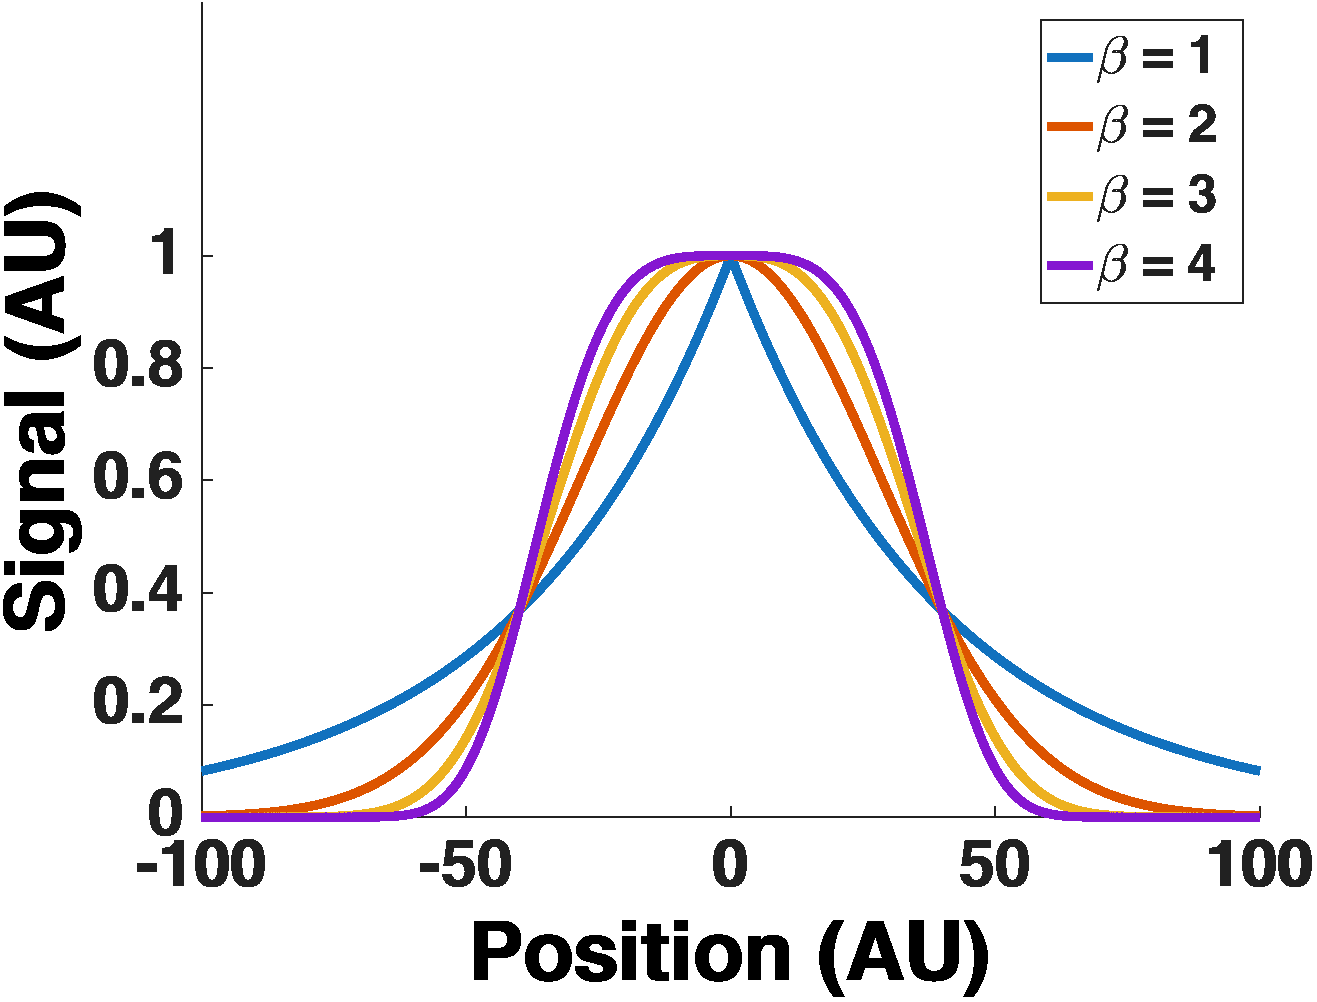
\includegraphics[height=3.8cm,keepaspectratio]{figures/gg_model_a.pdf}\end{subfigure}\hspace{0.02\linewidth}%
\begin{subfigure}[t]{0.38\linewidth}\centering\captionsetup{margin={6.25mm,0mm}}\caption{Model fits to MIP}\label{fig:gg_model_b}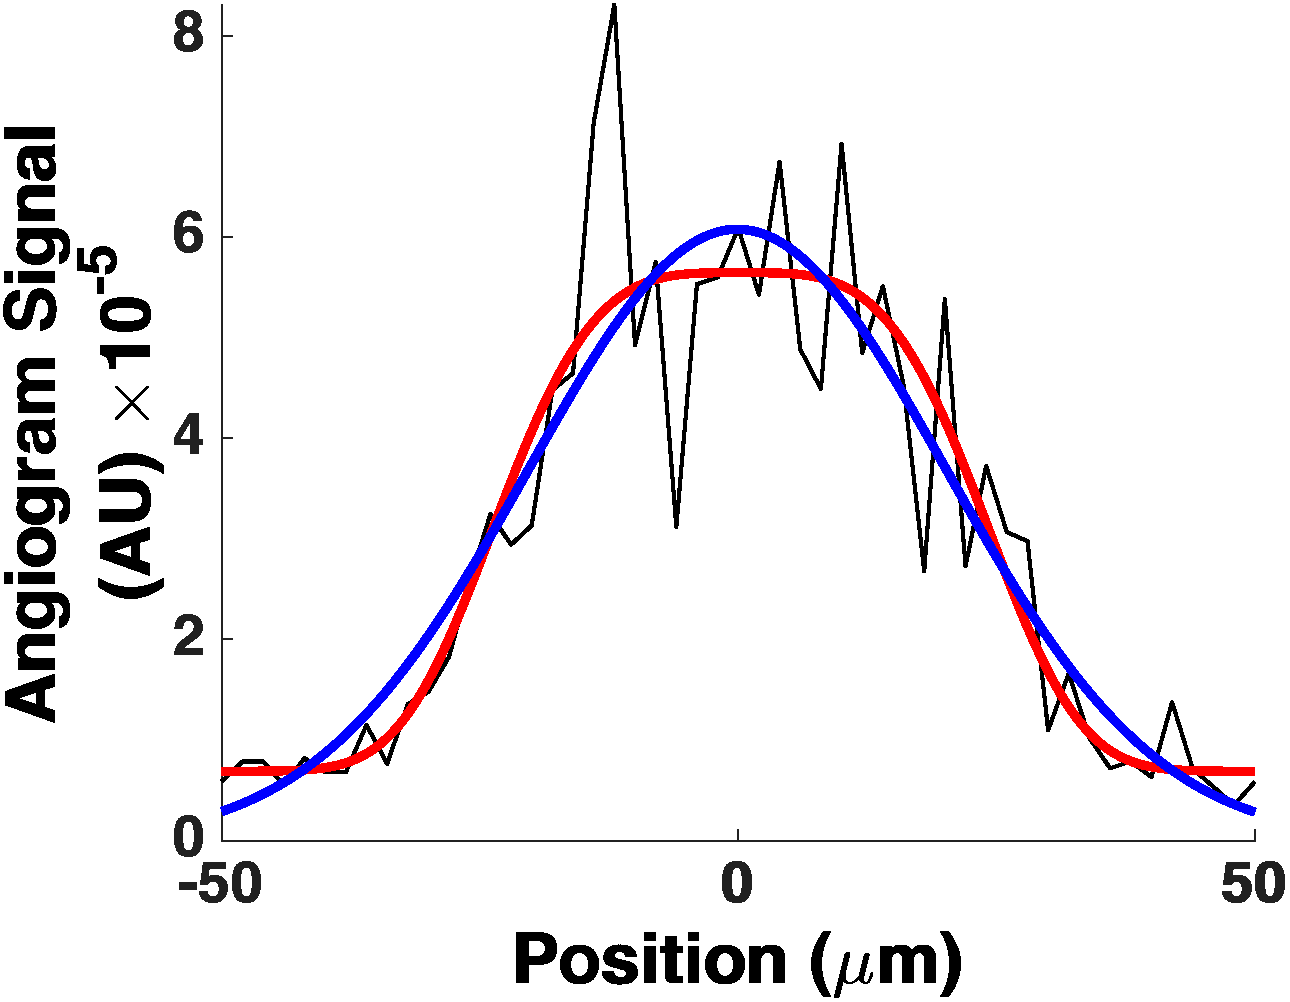
\includegraphics[height=3.8cm,keepaspectratio]{figures/gg_model_c.pdf}\end{subfigure}
\caption{(a) GG function for shape parameters $\beta = 1$, 2, 3, and 4.~(b) Example vessel intensity profile (black) taken from a MIP, with standard Gaussian (blue) and GG (red) fits. The MIP profile is flat-topped ($\beta = 9.9$), a shape the standard Gaussian cannot represent.}
\label{fig:gg_model}
\end{figure}

Two standard width metrics were calculated from the fitted models: the full width at half maximum (FWHM) and the $1/e^2$ width. For the standard Gaussian fit, the $1/e^2$ width was calculated as:
\begin{equation}
\label{eq:gauss_1e2}
w_{1/e^2,\,\mathrm{G}} = 4\sigma
\end{equation}
The FWHM for a Gaussian is related to the $1/e^2$ width by a fixed proportionality:
\begin{equation}
\label{eq:gauss_fwhm}
w_{fwhm,\,\mathrm{G}} = 2\sigma\sqrt{2\ln 2} = \frac{\sqrt{2\ln 2}}{2} \; w_{1/e^2,\,\mathrm{G}}
\end{equation}
and therefore only the $1/e^2$ width was calculated directly from the fit, with the FWHM obtainable via this known relationship.

For the GG fit, no such linear relationship exists between the FWHM and $1/e^2$ width, since both depend on the shape parameter $\beta$. Both metrics were therefore calculated independently as:
\begin{equation}
\label{eq:gg_fwhm}
w_{fwhm,\,\mathrm{GG}} = 2\alpha{\left(\ln 2\right)}^{1/\beta}
\end{equation}
\begin{equation}
\label{eq:gg_1e2}
w_{1/e^2,\,\mathrm{GG}} = 2\alpha \cdot 2^{1/\beta}
\end{equation}

\subsubsection{Binary mask based vessel diameter calculation}
\label{subsubsec:binary_mask}
For comparison with OCTA processing pipelines that rely on image binarisation, vessel diameters were also measured from binary masks generated by global thresholding. To determine the threshold level, the maximum angiogram intensity was measured after applying a 3D averaging filter with a kernel size of 50~$\times$~50~$\times$~10 voxels (lateral~$x$~$\times$~axial~$z$~$\times$~temporal~$t$) to the DyC-OCT angiogram volumes to reduce noise and minimize the effects of outliers. To produce a binarised black and white (BW) mask, the maximum angiogram intensity within these smoothed volumes were calculated, and five different threshold values were defined as fixed percentages of these maxima for MIP and MeIP. For MIP, the thresholds were defined as BW-1~=~40\%, BW-2~=~50\%, BW-3~=~60\%, BW-4~=~70\%, and BW-5~=~80\%. While for MeIP, the thresholds were defined as BW-1~=~07\%, BW-2~=~08\%, BW-3~=~09\%, BW-4~=~10\%, and BW-5~=~11\%.~These thresholds were selected empirically to cover the usable range of each projection. The upper and lower bounds were selected based on the point at which vessels began to be lost, and at which background noise and tissue signal were increasingly included, respectively. Each threshold was applied to the unsmoothed en face projection (MIP and MeIP) to generate a binary mask, and the vessel diameter was measured as the number of pixels above the threshold across the lateral vessel cross-section.

\subsubsection{Statistical analysis}
\label{subsubsec:stats}
To evaluate the accuracy and precision of all diameter measurement approaches, the calculated diameter values were plotted against the ground truth for each vessel across three conditions: pre-contrast, peak contrast, and post-contrast. A linear regression was fitted to each condition, yielding the slope ($m$) and coefficient of determination ($R^2$). A slope of $m = 1$ indicated perfect agreement with the ground truth, and $R^2$ quantified the goodness of fit of the linear model. Additionally, the coefficient of variation (CoV) was computed for each vessel across the time samples within each contrast condition and then averaged across vessels, to assess measurement precision (repeatability). For the model-based methods, six combinations were evaluated: two projection methods (MIP and MeIP) by three width metrics ($w_{1/e^2,\,\mathrm{G}}$, $\mathrm{FWHM}_{\mathrm{GG}}$, and $w_{1/e^2,\,\mathrm{GG}}$). For the binary mask based method, diameter was measured at five threshold levels (BW-1 through BW-5) for both MIP and MeIP. For the functional flicker stimulation experiment, a paired t-test was used to evaluate if stimulation induced changes were significant, and the Pearson correlation coefficient ($\rho$) between measured diameter values and angiogram intensity was computed for each method and vessel to assess whether the diameter measurements were affected by changes in angiogram intensity. Measurements with $p < 0.05$ were considered statistically significant (significance levels: $^{*}p < 0.05$, $^{**}p < 0.01$, $^{***}p < 0.001$). A paired t-test was used to evaluate whether vessel diameters differed significantly between the pre- and post-stimulation windows.

\section{Results}
% Results

\subsection{Qualitative assessment of vessel underestimation}
\label{subsec:qualitative}

% \begin{figure}[htbp] 
% [htbp] = placement suggestion “try Here, otherwise Top, Bottom, or a dedicated Page" in that order
% \begin{figure}[H] 
% H = “Here definitely”, requires \usepackage{float}
% \centering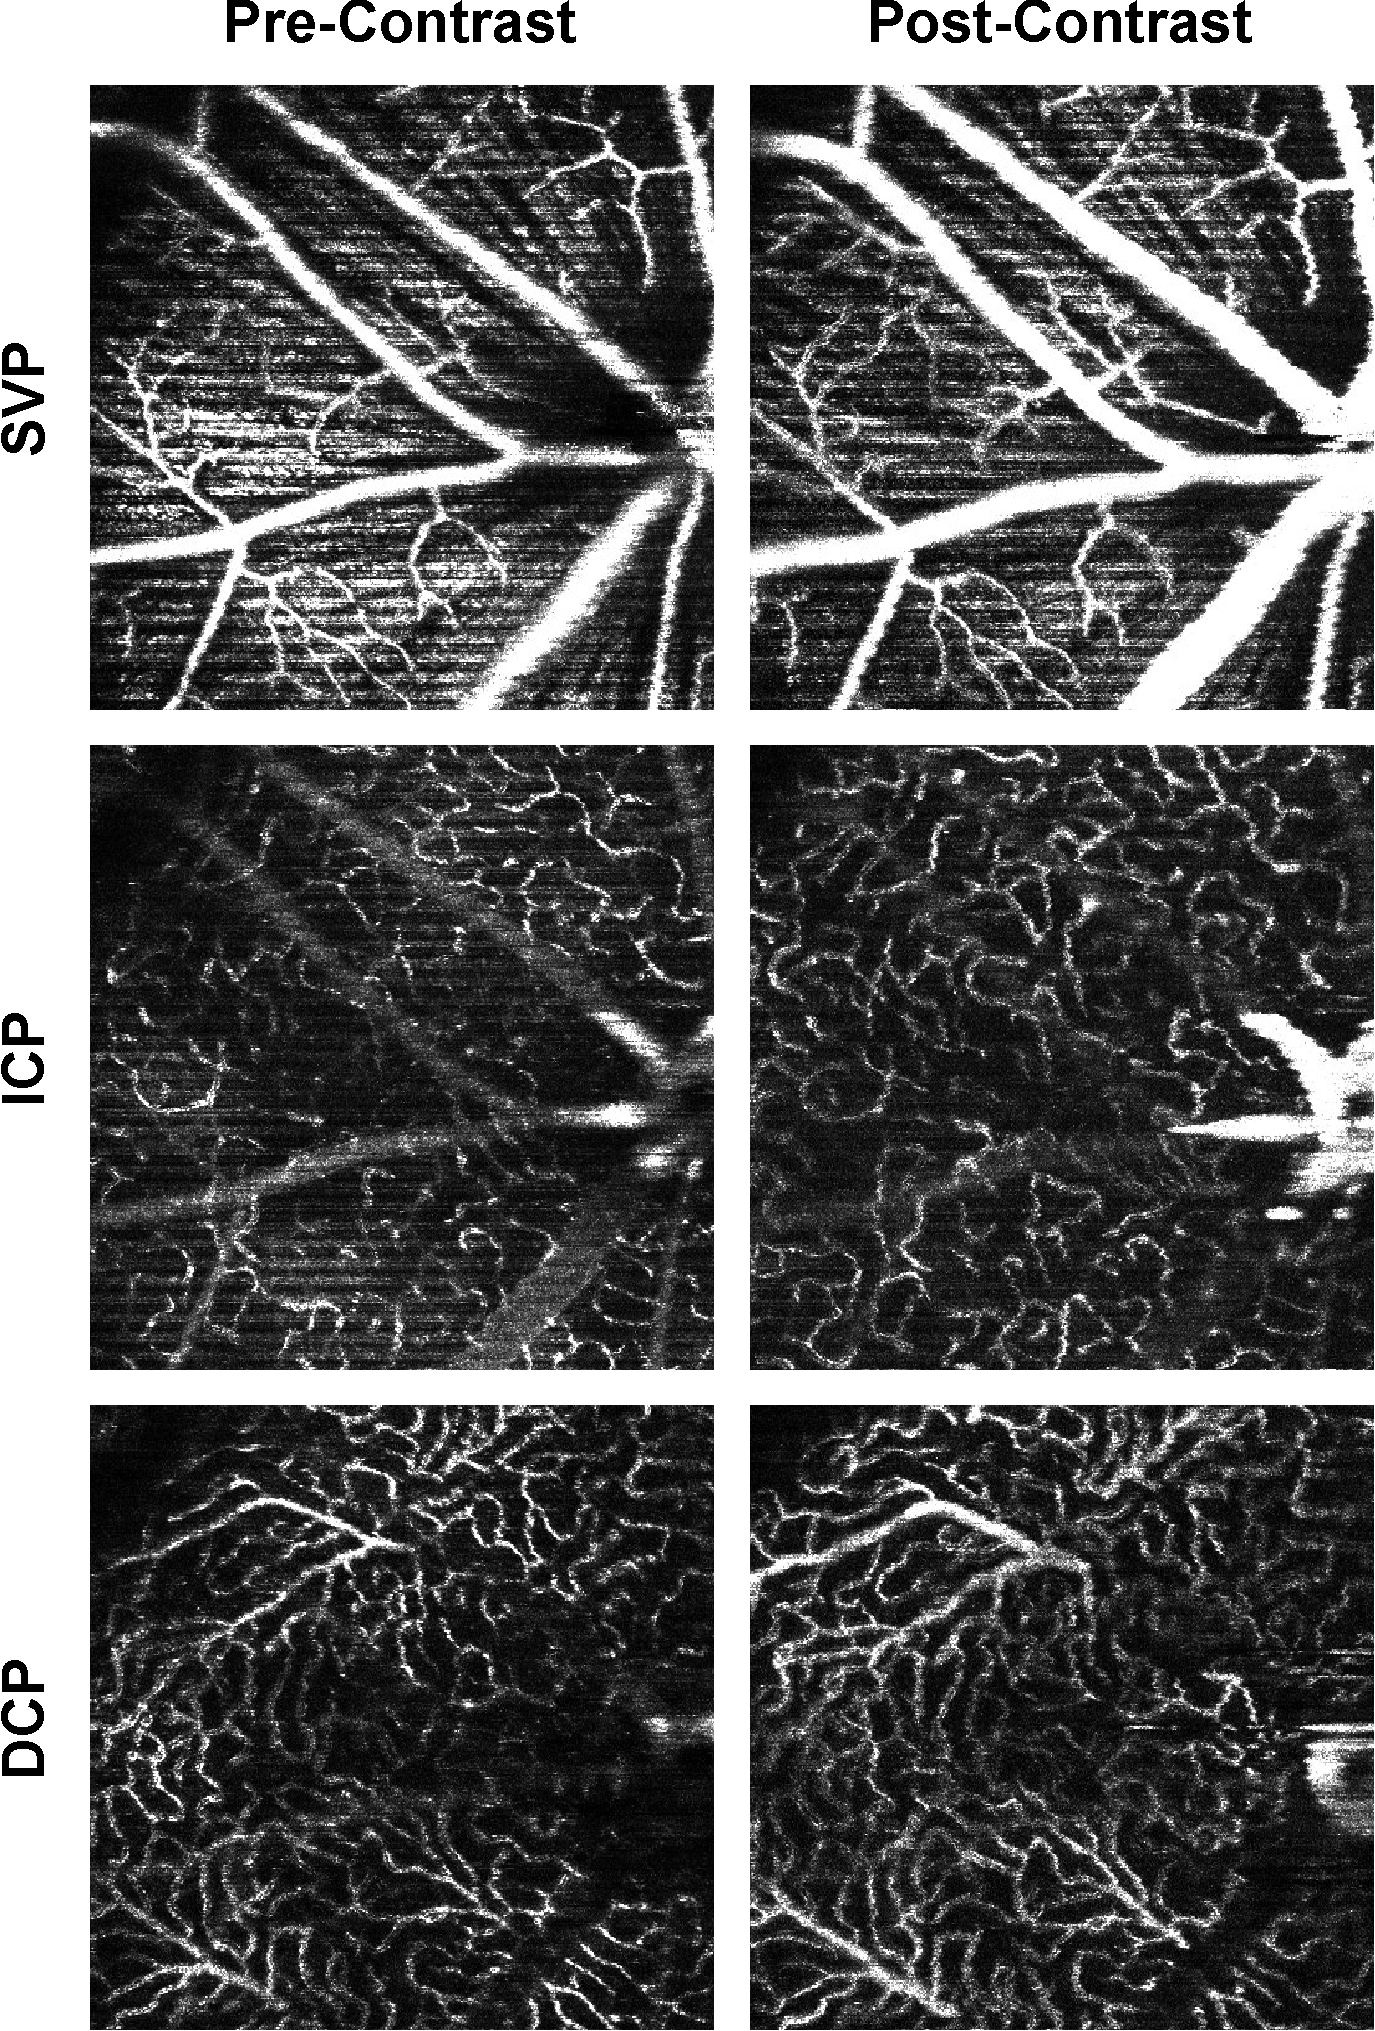
\includegraphics[width=\linewidth,height=\dimexpr\textheight-\pagetotal-3\baselineskip\relax,keepaspectratio]{figures/Figure_1.pdf} 
% height=\dimexpr\textheight-\pagetotal-#\baselineskip\relax = set the figure height to the remaining space on the page, accounting for the current vertical position and leaving room for caption and label.
    % \dimexpr = allow for dynamic calculation of figure height based on the remaining space on the page.
    % -\pagetotal = account for the vertical space already used on the page, ensuring the figure does not exceed the remaining space.
    % -#\baselineskip = leave room for the figure caption and label, which typically require a few lines of text. Adjust the number of baselineskip (#) as needed to ensure the figure fits well without excessive whitespace.
    % \relax = allow the figure to scale down if necessary to fit within the specified height while maintaining aspect ratio.
% \label{fig:enface}
% \end{figure}

\begin{figure}[H] 
\centering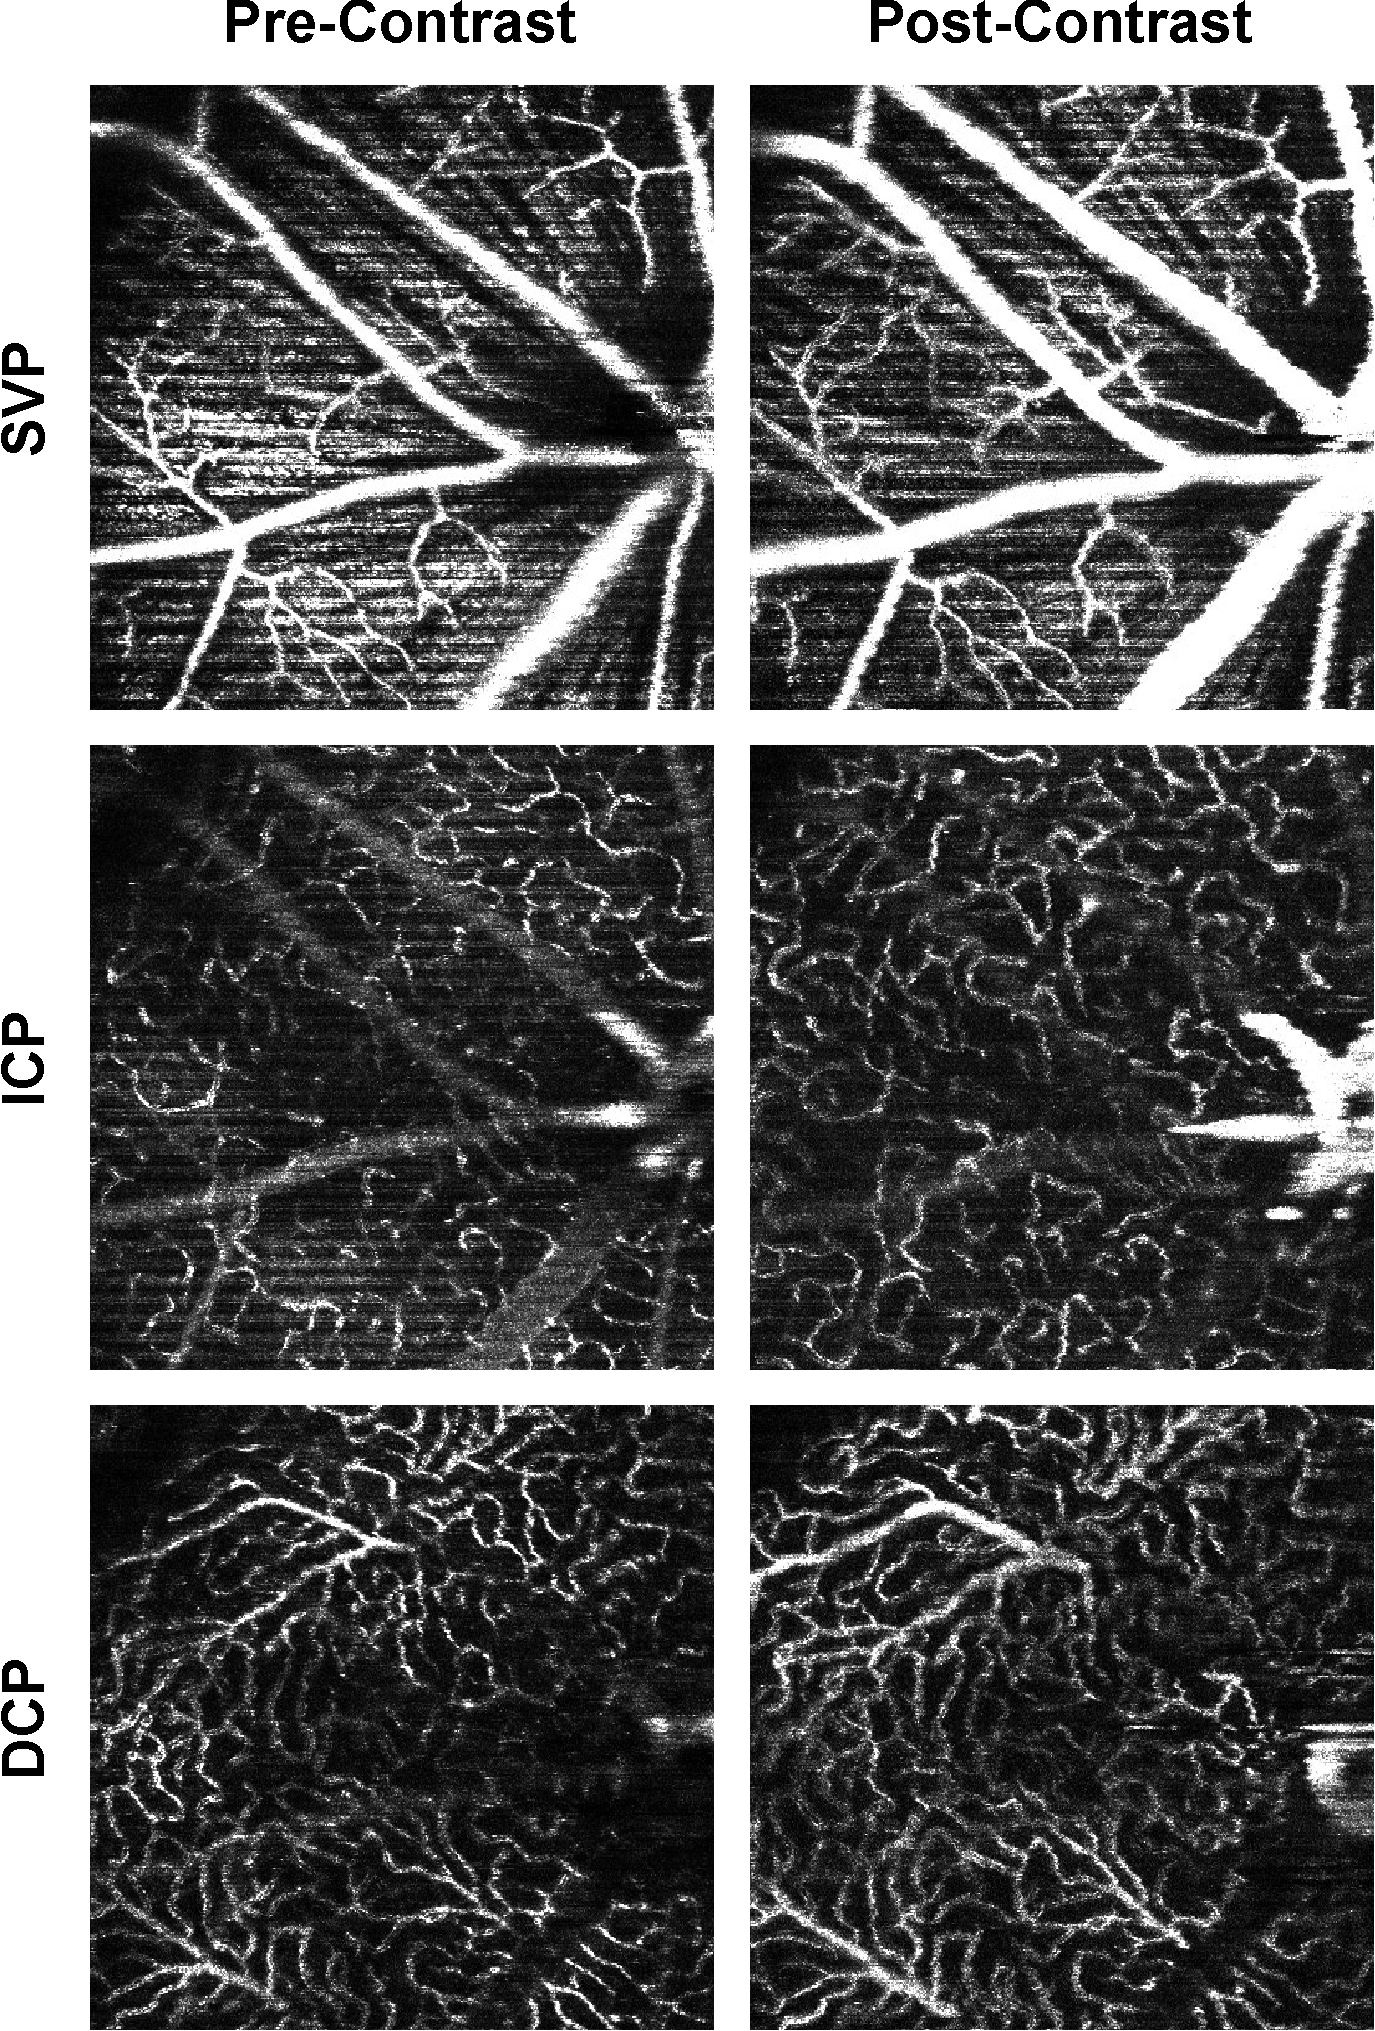
\includegraphics[width=0.45\linewidth,keepaspectratio]{figures/Figure_1.pdf} 
\caption{OCTA MIP en face of the SVP, ICP, and DCP before (left) and after (right) the administration of Intralipid 20\%. Vessels appear visibly wider and brighter post-contrast across all layers, most prominently in the larger vessels.}
\label{fig:enface}
\end{figure}

Figure~\ref{fig:enface} shows OCTA MIP en face of the superficial vascular plexus (SVP), intermediate capillary plexus (ICP), and deep capillary plexus (DCP) before and after contrast injection. Across all three layers, vessels appeared visibly wider and brighter post-contrast injection, consistent with previous literature showing that OCTA underestimates vessel diameter in the absence of a contrast agent~\cite{merkleHighresolutionDepthresolvedVascular2021}. This effect was most pronounced in the larger vessels, especially in the SVP, where the major retinal arteries and veins appeared noticeably thicker after contrast administration. In the ICP and DCP, the capillary networks also showed improved visibility, though the effect was less dramatic.

DyC OCTA projections helped visualise the temporal changes in vessel diameter pre- and post-contrast injection (Fig.~\ref{fig:dycoct}). Pre-contrast injection, the vessel cross-sections appeared narrower than their true diameter (Fig.~\ref{fig:dycoct}a), which could be due to lateral edge signal suppression by the RBC orientation artefact~\cite{bernucciInvestigationArtifactsRetinal2018}.~\textcolor{red}{At peak contrast, the Intralipid filled the vascular lumen uniformly and showed the full extent of the vessel cross-section (Fig.~\ref{fig:dycoct}b). However, the high scattering nature of the contrast agent produced light diffusion beyond the vessel wall, resulting in an apparent vessel diameter that slightly exceeded the true anatomical diameter. In the post-contrast phase, the signal stabilised as the initial bolus cleared, and the vessel boundaries remained more visible than before injection without the overestimation observed at peak contrast (Fig.~\ref{fig:dycoct}c). The MIP and the corresponding binary mask over time (Figs.~\ref{fig:dycoct}d--e) showed the observed temporal changes in vessel diameter across the three phases. The mean OCTA intensity (Fig.~\ref{fig:dycoct}f) showed a sharp increase post-contrast injection, followed by a decrease to a new steady state that remained elevated above the pre-contrast baseline.} These observations confirm that the contrast agent does significantly enhance vessel visibility and diameter, and that the post-contrast images show improved vessel delineation compared to pre-contrast.

\begin{figure}[H]
\centering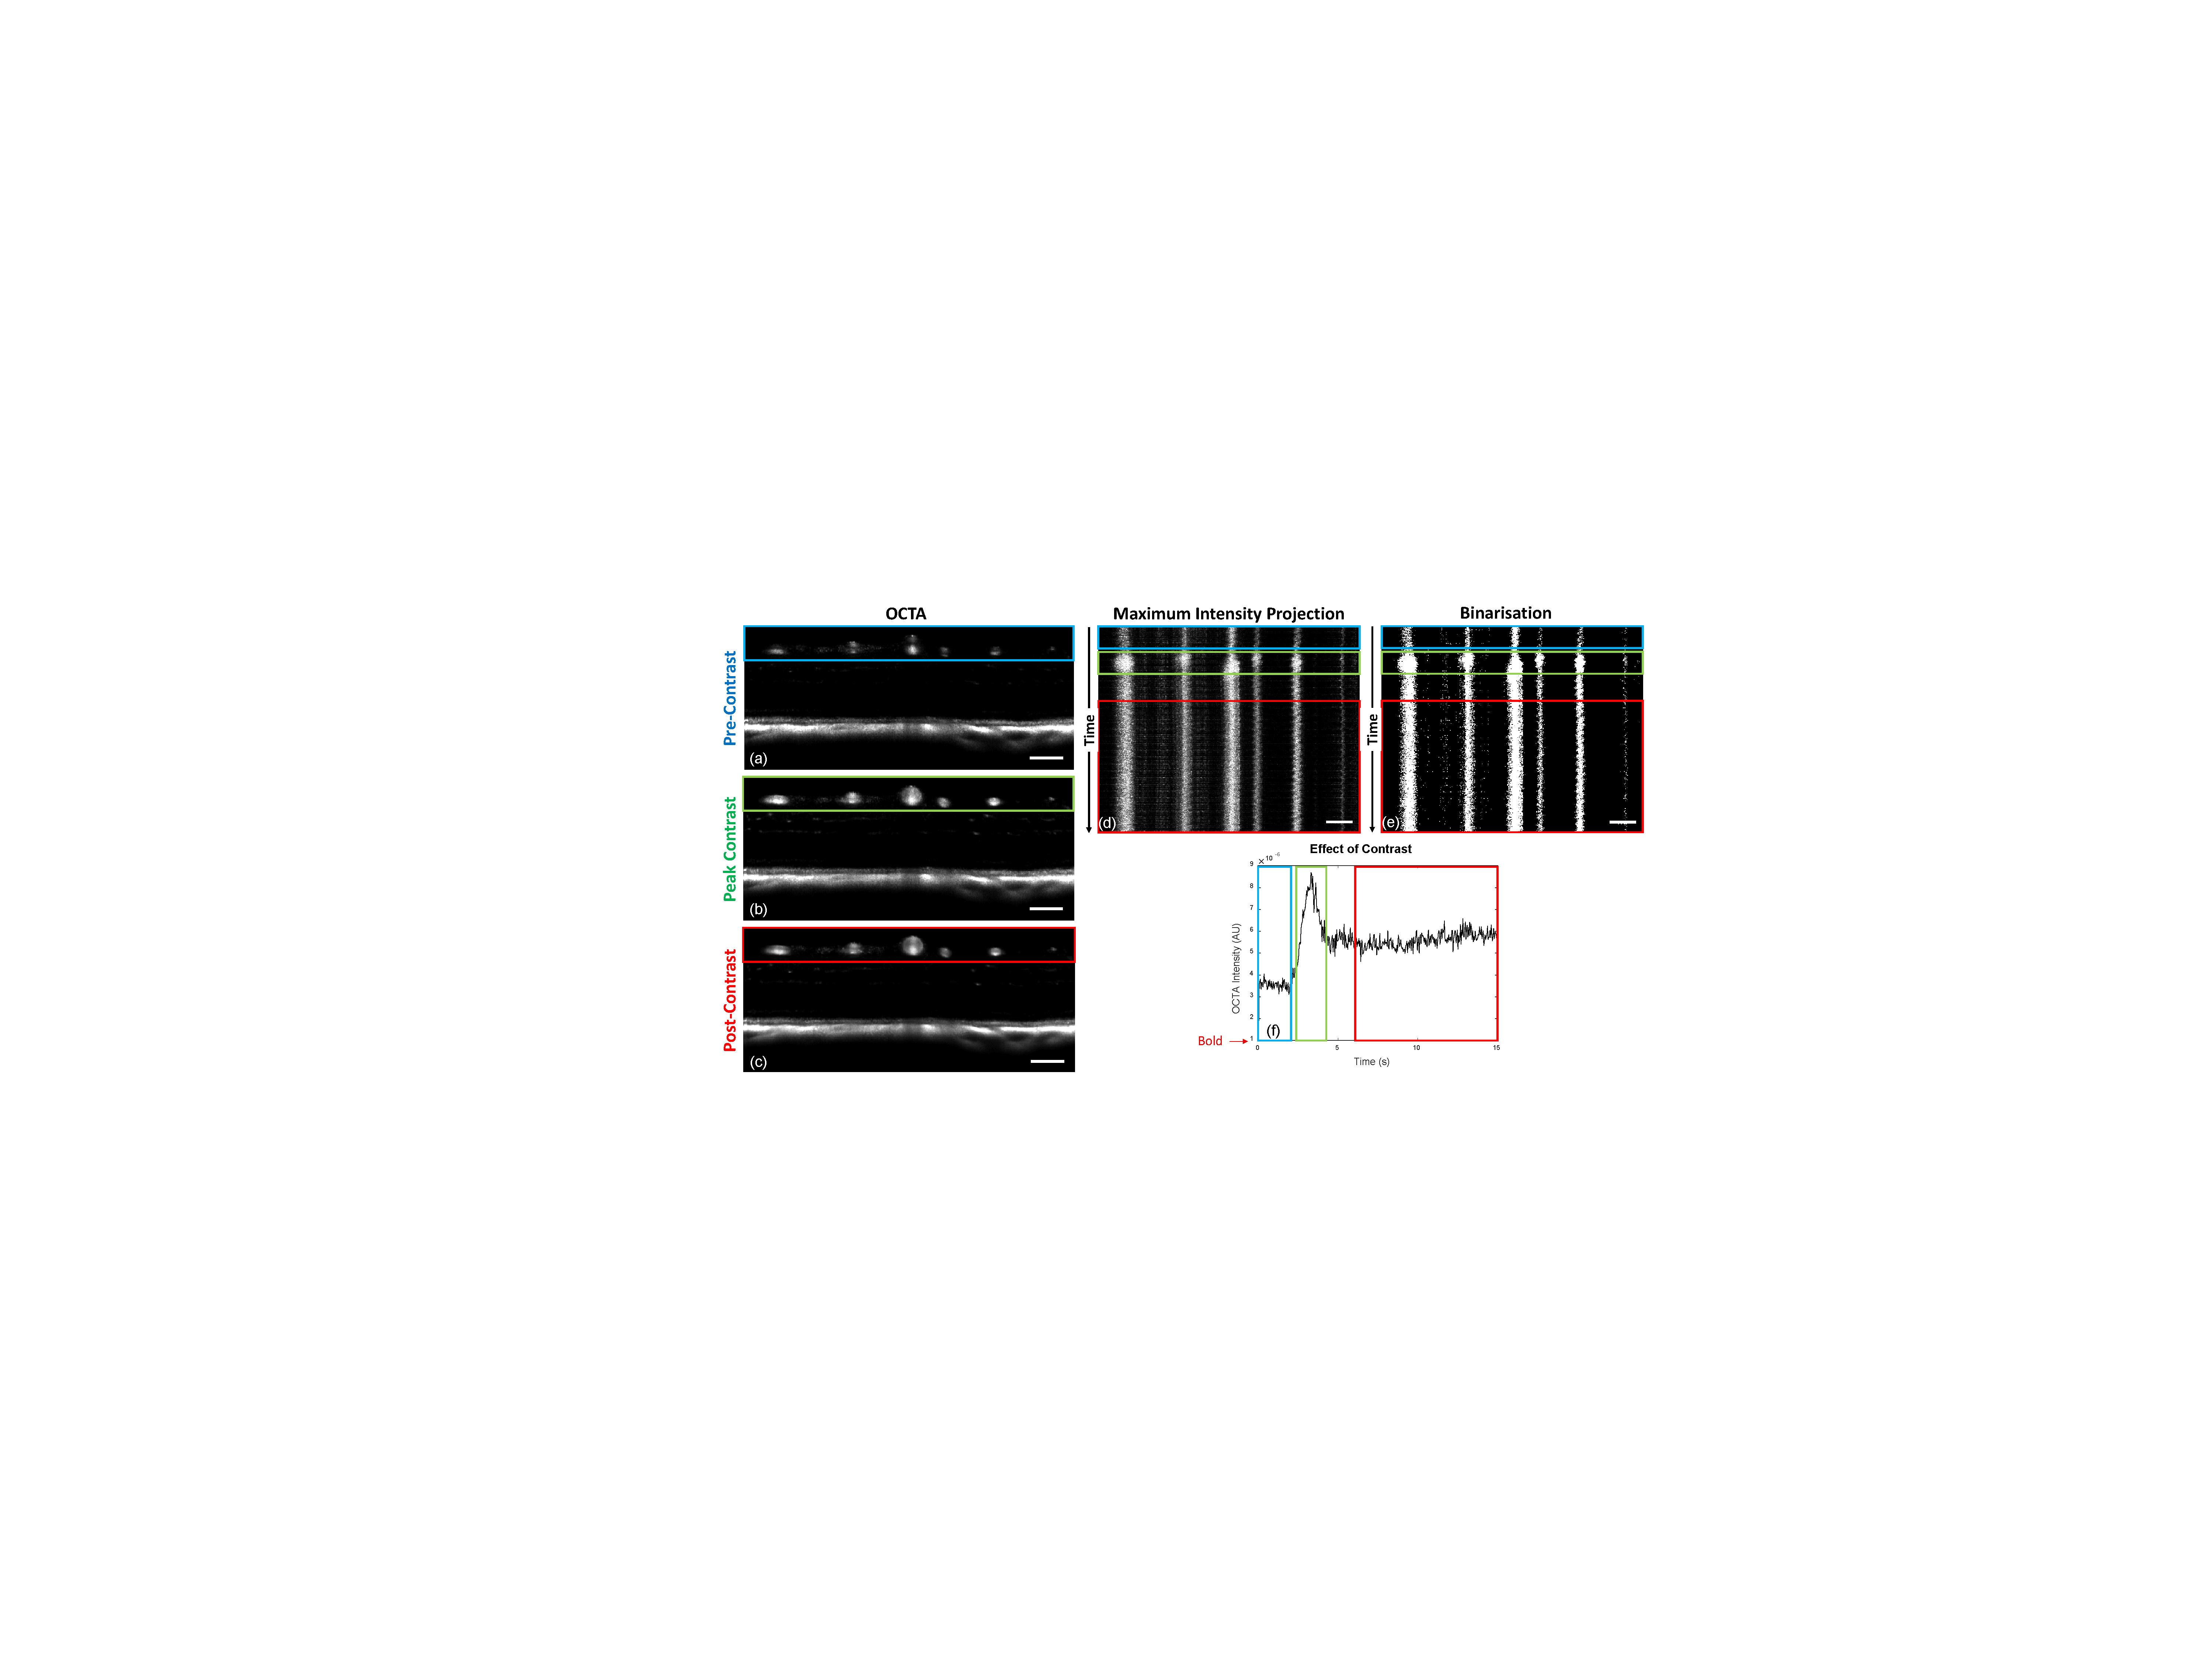
\includegraphics[width=\linewidth,height=\dimexpr\textheight-\pagetotal-8\baselineskip\relax,keepaspectratio]{figures/Figure_2.pdf}
\caption{DyC-OCT B-scan angiograms at (a) pre-contrast, (b) peak contrast, and (c) post-contrast timepoints.~(d) MIP and (e) binarisation of the vessel cross-sections over time, with coloured boxes indicating the pre-contrast (blue), peak-contrast (green), and post-contrast (red) windows.~(f) Mean OCTA intensity over time, showing the temporal intensity dynamics.~\textcolor{red}{All scale bars are 100\,\textmu{}m.}}
\label{fig:dycoct}
\end{figure}

\subsection{Accuracy and linearity of diameter measurements}
\label{subsec:linearity_accuracy_model}
To evaluate the accuracy and linearity of all diameter measurement approaches, the calculated diameter values were plotted against the ground truth for each vessel across three conditions: pre-contrast, peak contrast, and post-contrast. A linear regression was fitted to each condition, yielding the slope ($m$) and coefficient of determination ($R^2$), which are summarised in Table~\ref{tab:accuracy_linearity}. A slope of $m = 1$ (black line) indicated perfect agreement with the ground truth, and $R^2$ quantified the goodness of fit of the linear model. For the model-based methods, six combinations were evaluated: two projection methods (MIP and MeIP) by three width metrics ($w_{1/e^2,\,\mathrm{G}}$, $\mathrm{FWHM}_{\mathrm{GG}}$, and $w_{1/e^2,\,\mathrm{GG}}$; Fig.~\ref{fig:scatter_model}). For the binarisation-based methods, diameter was measured at five threshold levels (BW-1 through BW-5) for both MIP (Fig.~\ref{fig:scatter_bw_mip}) and MeIP (Fig.~\ref{fig:scatter_bw_meip}). 

\begin{figure}[H]
\centering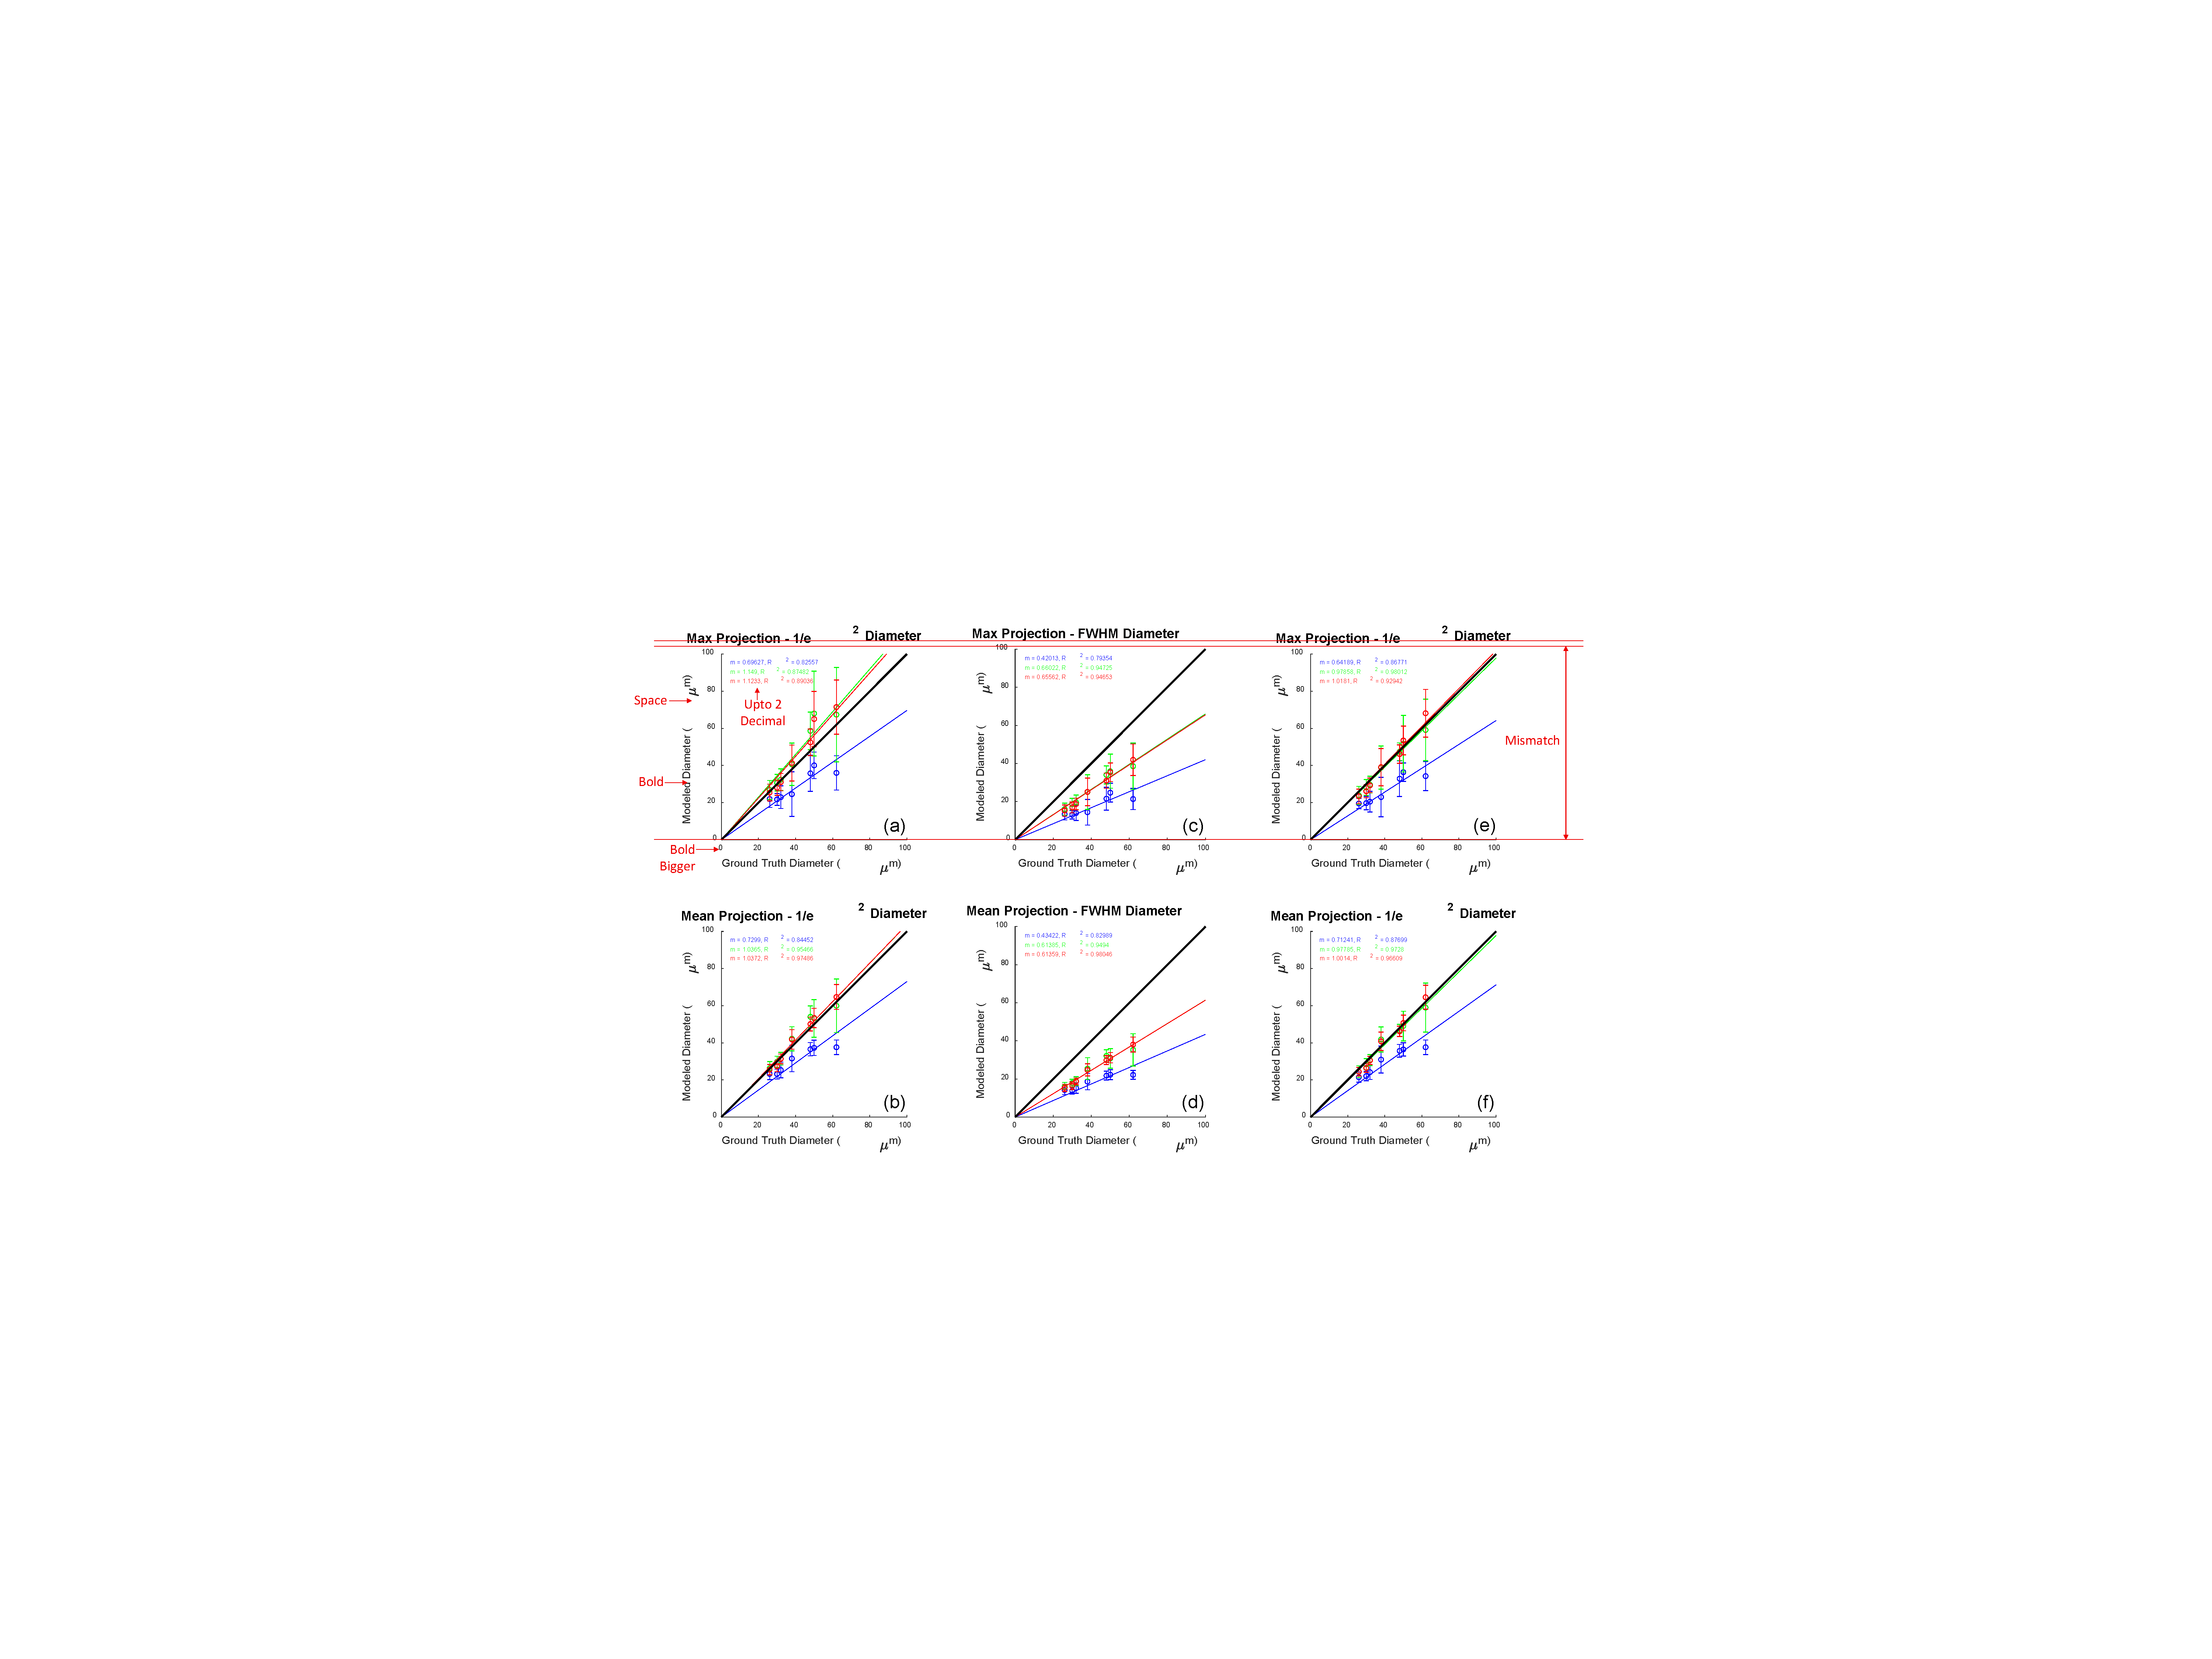
\includegraphics[width=\linewidth,height=\dimexpr\textheight-\pagetotal-8\baselineskip\relax,keepaspectratio]{figures/Figure_4.pdf}
\caption{Modelled versus ground truth vessel diameter using MIP (top row) and MeIP (bottom row). Columns correspond to (a,b) Gaussian $1/e^2$ width, (c,d) GG FWHM, and (e,f) GG $1/e^2$ width. Regression lines and statistics are shown for pre-contrast (blue), peak contrast (green), and post-contrast (red) conditions. The black line indicates the identity line ($m = 1$).}
\label{fig:scatter_model}
\end{figure}

All model-based methods underestimated vessel diameter in pre-contrast data, with slopes ranging from 0.42 to 0.73 (Table~\ref{tab:accuracy_linearity}). Contrast enhancement improved accuracy across all metrics, though the degree of improvement varied. The $\mathrm{FWHM}_{\mathrm{GG}}$ metric remained well below unity even post-contrast. The $w_{1/e^2,\,\mathrm{G}}$ with MIP slightly overestimated post-contrast ($m = 1.12$--$1.15$), while MeIP yielded values closer to unity ($m = 1.04$). The $w_{1/e^2,\,\mathrm{GG}}$ with MeIP provided the best overall agreement, achieving a slope closest to unity with $m = 1.001$ ($R^2 = 0.97$) post-contrast, which was the closest to the identity line of all tested model-based methods. Across all metrics, MeIP mostly outperformed MIP in both accuracy and linearity (Table~\ref{tab:accuracy_linearity}, Fig.~\ref{fig:scatter_model}).

\begin{figure}[htbp]
\centering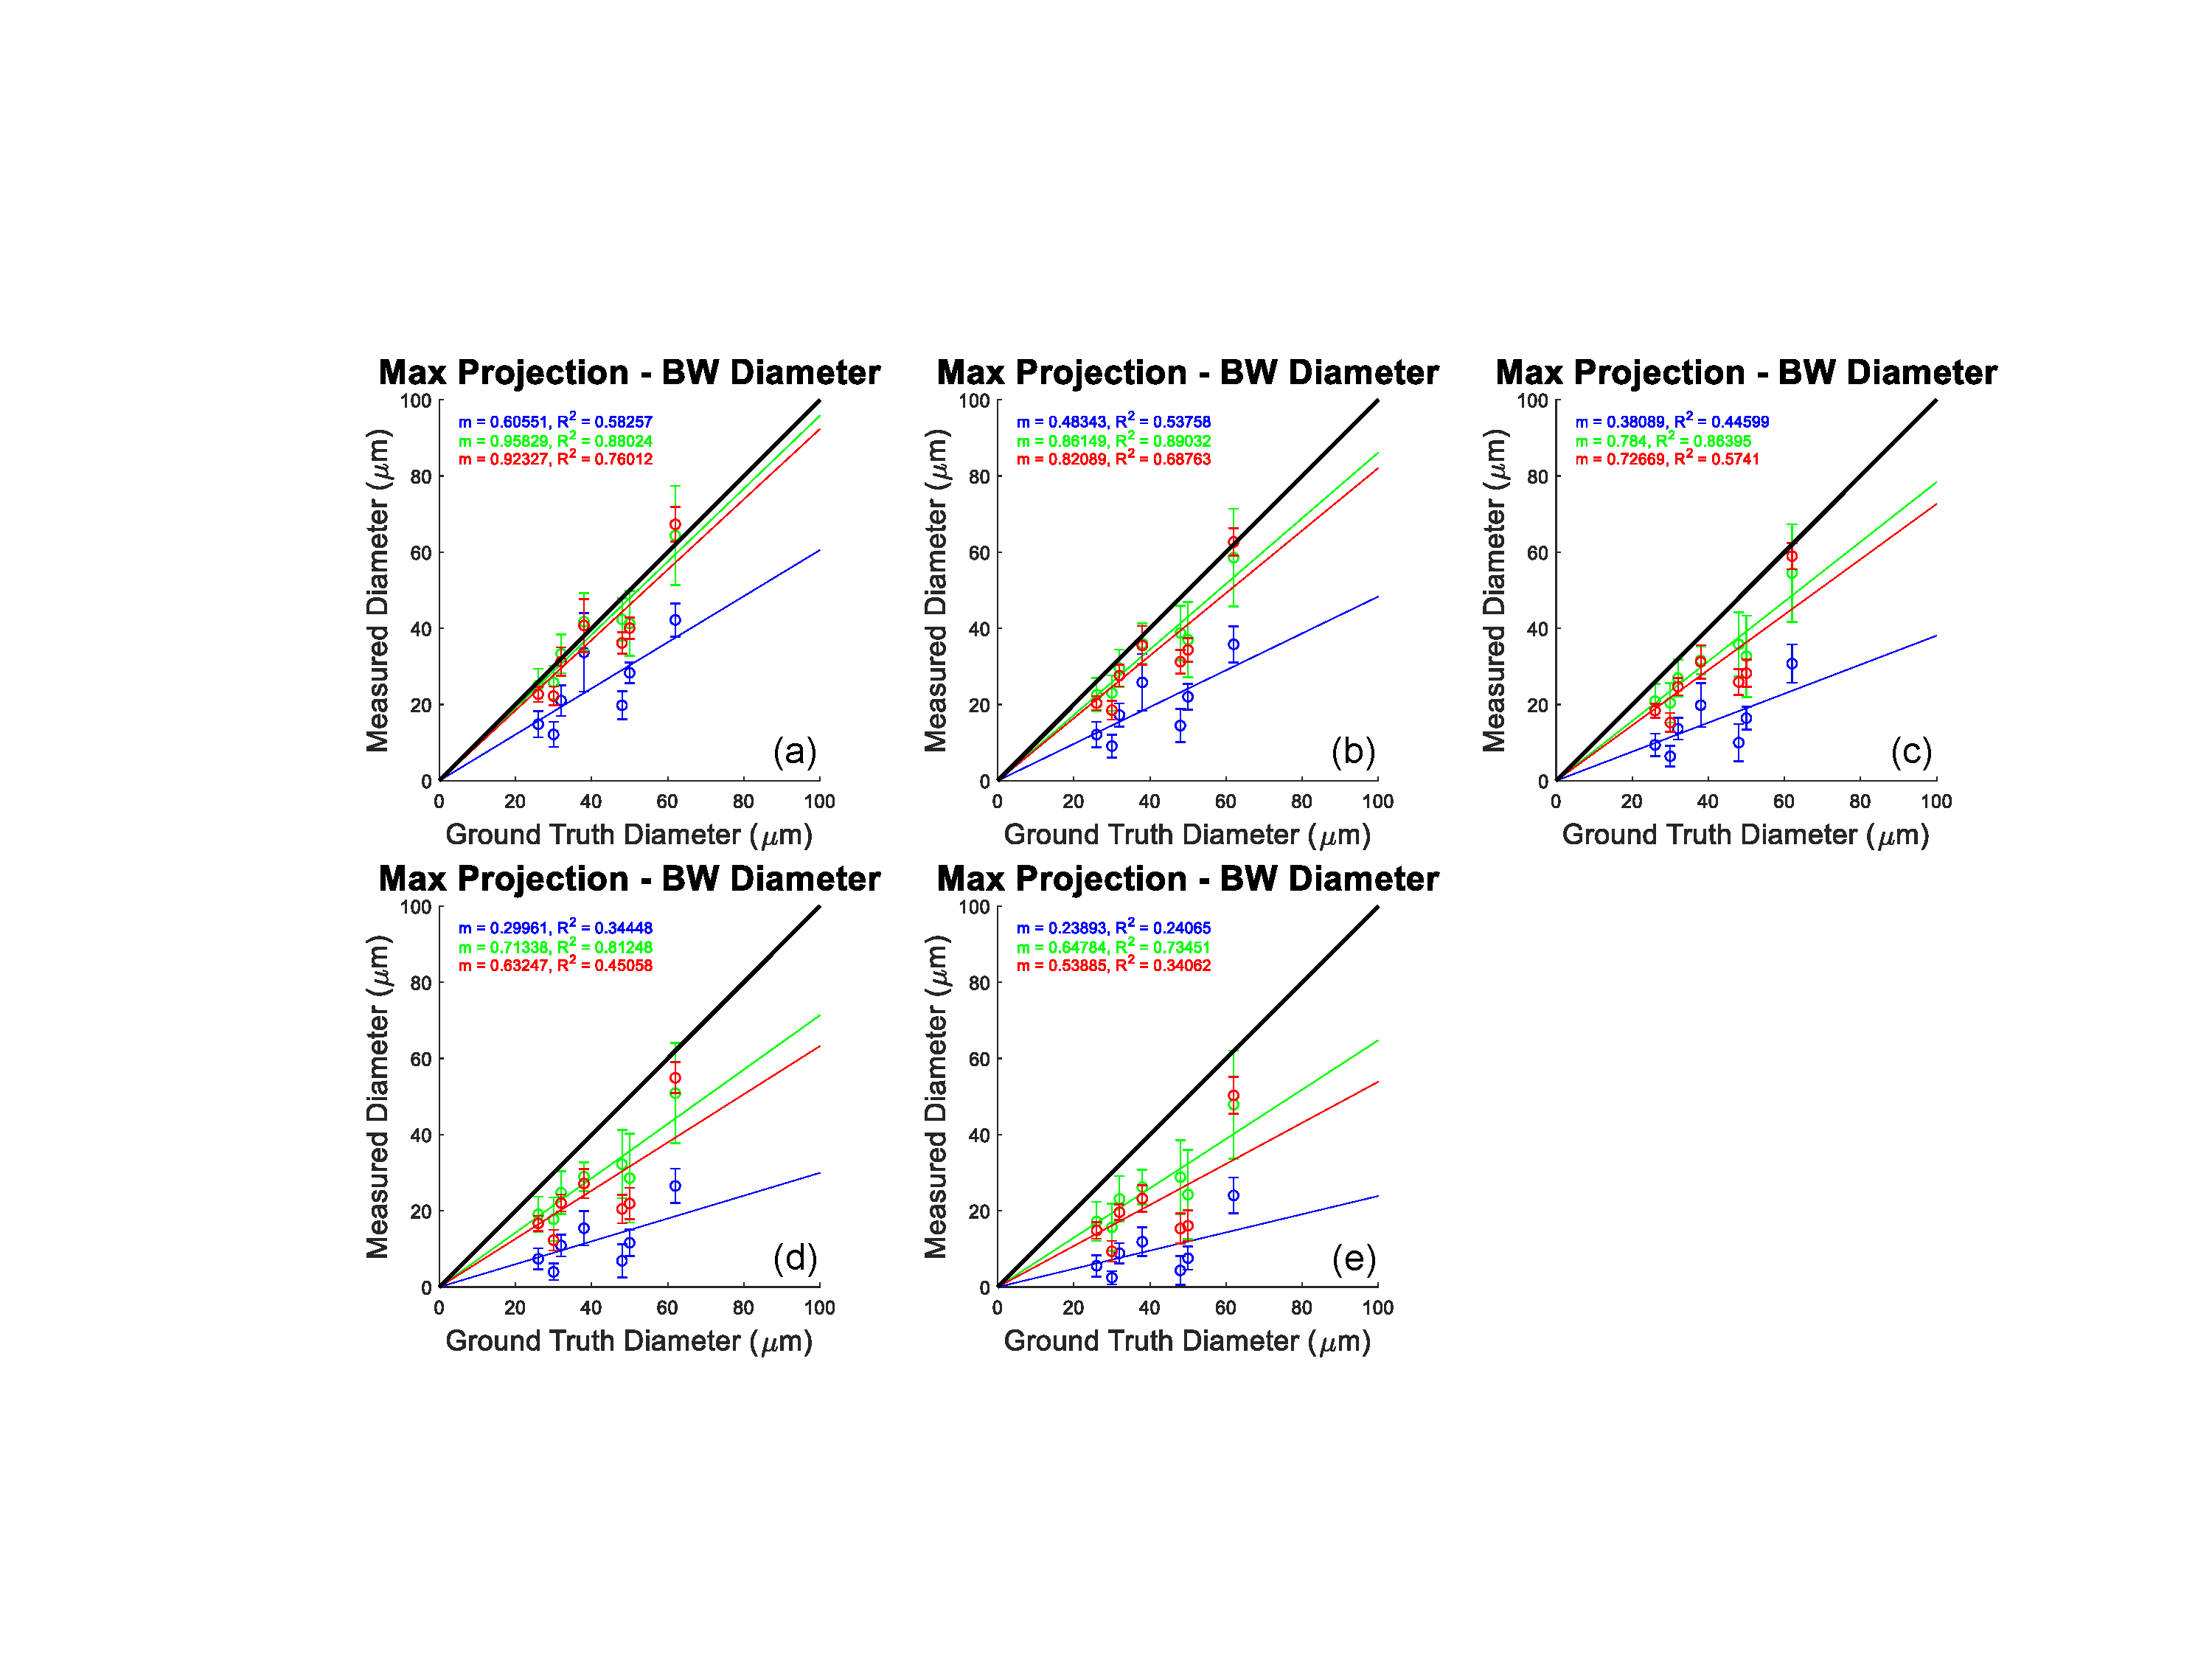
\includegraphics[width=\linewidth,keepaspectratio]{figures/Figure_5.pdf}
\caption{Vessel diameter measured from BW images versus ground truth for MIP at five threshold levels: (a) BW-1 through (e) BW-5. Regression lines and statistics are shown for pre-contrast (blue), peak contrast (green), and post-contrast (red). Both slope $m$ and $R^2$ decrease with increasing threshold values.}
\label{fig:scatter_bw_mip}
\end{figure}

\begin{figure}[htbp]
\centering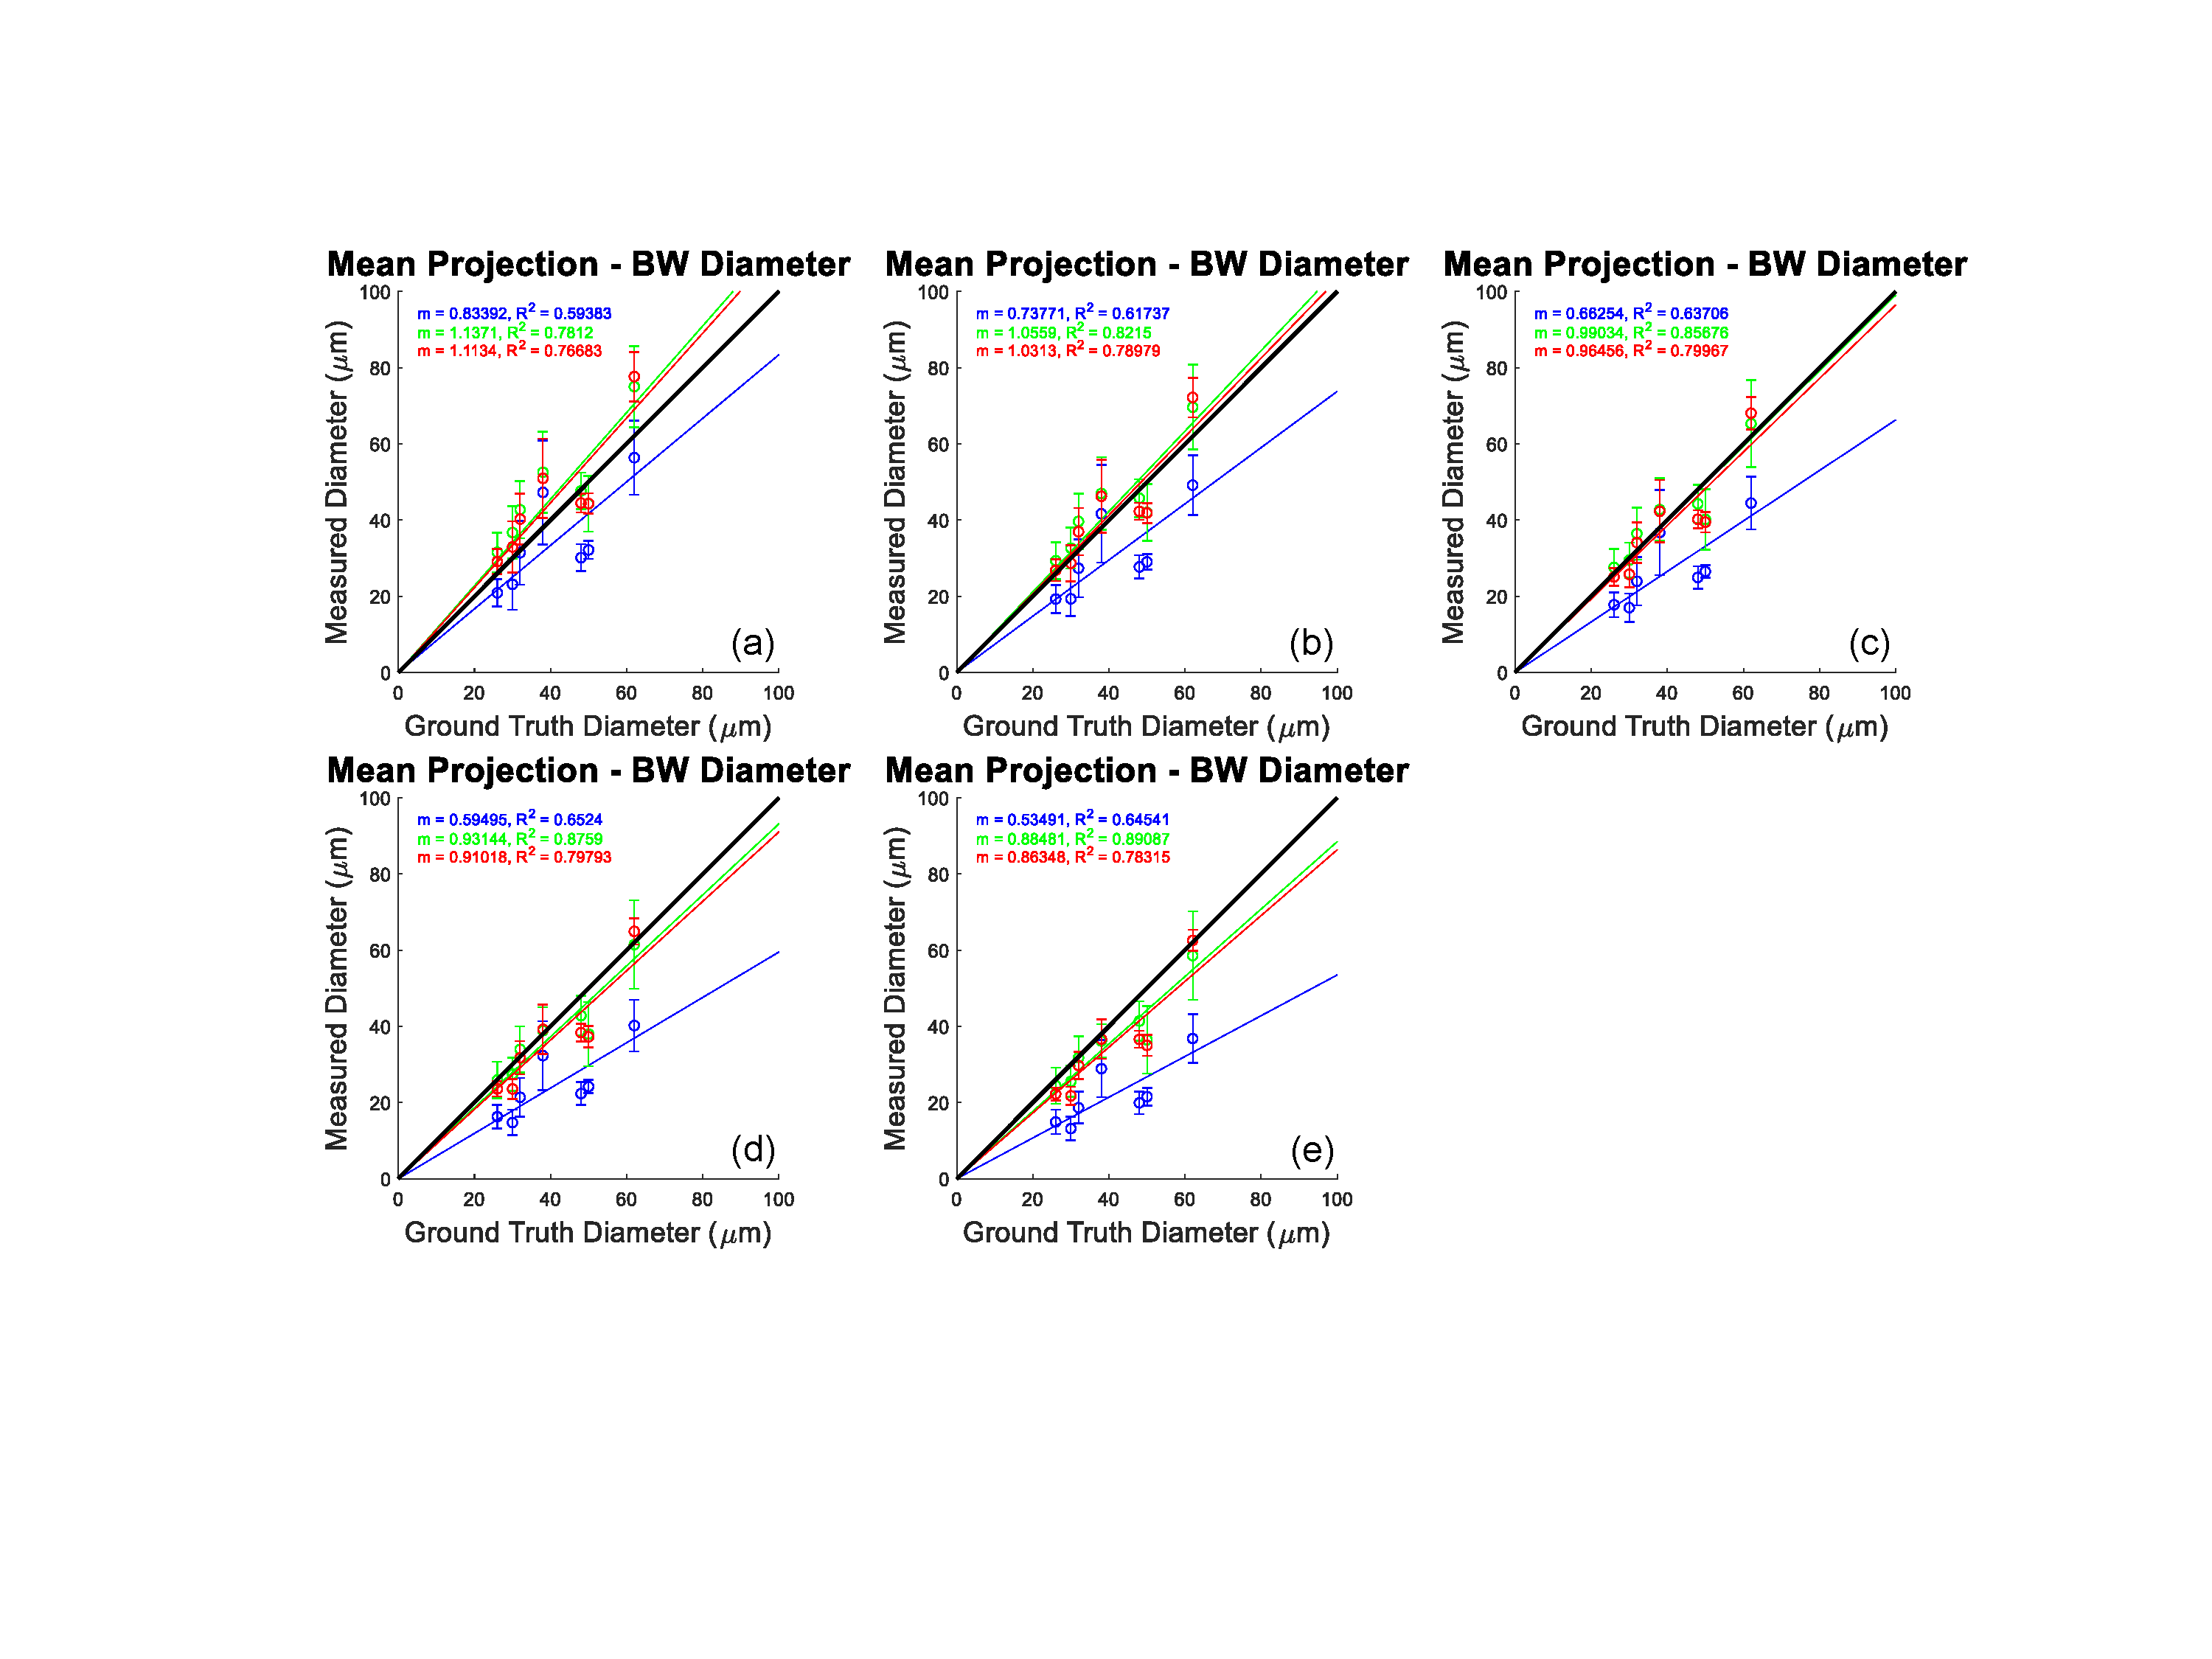
\includegraphics[width=\linewidth,keepaspectratio]{figures/Figure_6.pdf}
\caption{Vessel diameter measured from BW images versus ground truth for MeIP at five threshold levels: (a) BW-1 through (e) BW-5. Regression lines and statistics are shown for pre-contrast (blue), peak contrast (green), and post-contrast (red) conditions. MeIP yielded higher slopes and more stable $R^2$ values compared to MIP (Fig.~\ref{fig:scatter_bw_mip}).}
\label{fig:scatter_bw_meip}
\end{figure}

For binarisation-based methods, the slope decreased with increase in threshold values across all contrast conditions and projections (Table~\ref{tab:accuracy_linearity}). MeIP $m$ values were consistently higher than MIP across all threshold and contrast conditions. Also, across all contrast conditions, $m$ dropped more significantly with increase in threshold for MIP than for MeIP. For MIP, the pre- and post-contrast $R^2$ decreased substantially with increase in threshold, whereas for MeIP, the $R^2$ remained relatively stable. At lower threshold values and at peak and post-contrast, MeIP overestimated the vessel diameter more than MIP. At peak and post-contrast, MeIP BW-3 achieved a slope of $m = 0.99$ and $m = 0.97$ respectively, though with a lower $R^2 = 0.86$ and $R^2 = 0.80$ respectively, compared to $w_{1/e^2,\,\mathrm{GG}}$ which achieved $m = 1.001$ with a higher $R^2 = 0.97$. Overall, MeIP provided more reliable binarisation-based diameter measurements than MIP.

\begin{table}[htbp]
\caption{Summary of slope ($m$) and coefficient of determination ($R^2$) for all diameter measurement methods across pre-contrast, peak contrast, and post-contrast conditions. Methods are grouped as binarisation-based and model-based. Bold slope values indicate agreement within 10\% of unity ($0.9 \leq m \leq 1.1$).}
\label{tab:accuracy_linearity}
\centering
\resizebox{\textwidth}{!}{%
\begin{tabular}{l c c | c c | c c | c c | c c || c c | c c | c c}
\hline
 & \multicolumn{2}{c|}{\textbf{BW-1}} & \multicolumn{2}{c|}{\textbf{BW-2}} & \multicolumn{2}{c|}{\textbf{BW-3}} & \multicolumn{2}{c|}{\textbf{BW-4}} & \multicolumn{2}{c||}{\textbf{BW-5}} & \multicolumn{2}{c|}{\textbf{$w_{1/e^2,\,\mathrm{G}}$}} & \multicolumn{2}{c|}{\textbf{$\mathrm{FWHM}_{\mathrm{GG}}$}} & \multicolumn{2}{c}{\textbf{$w_{1/e^2,\,\mathrm{GG}}$}} \\
 & MIP & MeIP & MIP & MeIP & MIP & MeIP & MIP & MeIP & MIP & MeIP & MIP & MeIP & MIP & MeIP & MIP & MeIP \\
\hline
\multicolumn{17}{l}{\textit{Slope ($m$)}} \\
\hline
Pre  & 0.61 & 0.83 & 0.48 & 0.74 & 0.38 & 0.66 & 0.30 & 0.59 & 0.24 & 0.53 & 0.70 & 0.73 & 0.42 & 0.43 & 0.64 & 0.71 \\
Peak & \textbf{0.96} & 1.14 & 0.86 & \textbf{1.06} & 0.78 & \textbf{0.99} & 0.71 & \textbf{0.93} & 0.65 & 0.88 & 1.15 & \textbf{1.04} & 0.66 & 0.61 & \textbf{0.98} & \textbf{0.98} \\
Post & \textbf{0.92} & 1.11 & 0.82 & \textbf{1.03} & 0.73 & \textbf{0.97} & 0.63 & \textbf{0.91} & 0.54 & 0.86 & 1.12 & \textbf{1.04} & 0.66 & 0.61 & \textbf{1.02} & \textbf{1.00} \\
\hline
\multicolumn{17}{l}{\textit{Coefficient of determination ($R^2$)}} \\
\hline
Pre  & 0.58 & 0.59 & 0.54 & 0.62 & 0.45 & 0.64 & 0.34 & 0.65 & 0.24 & 0.65 & 0.83 & 0.84 & 0.79 & 0.83 & 0.87 & 0.88 \\
Peak & 0.88 & 0.78 & 0.89 & 0.82 & 0.86 & 0.86 & 0.81 & 0.88 & 0.74 & 0.89 & 0.87 & 0.95 & 0.95 & 0.95 & 0.98 & 0.97 \\
Post & 0.76 & 0.77 & 0.69 & 0.79 & 0.57 & 0.80 & 0.45 & 0.80 & 0.34 & 0.78 & 0.89 & 0.97 & 0.95 & 0.98 & 0.93 & 0.97 \\
\hline
\end{tabular}%
}
\end{table}

\subsection{Repeatability and linearity comparison across all methods}
\label{subsec:comparison_all_methods}
\textcolor{red}{(confirm the values reported here with the actual data, as these are just extracted from the bar plots.)}

To compare the repeatability and linearity across BW1--5 and the model based approach, the coefficient of variation (CoV) and $R^2$ were computed (Fig.~\ref{fig:cov_r2}). For MIP based measurements (Fig.~\ref{fig:cov_r2}a), the CoV of BW method increased with increase in threshold while the CoV of the model based methods remained relatively stable. With increase in threshold values BW1--5, the CoV increased from approximately 0.2 to 0.47 for pre-contrast, 0.17 to 0.32 for peak contrast, and 0.1 to 0.18 for post-contrast data. The model based methods (G-$e^2$, GG-HM, GG-$e^2$) exhibited CoV values of approximately 0.24--0.27 for pre-contrast data, with reduced values of approximately 0.16--0.18 post-contrast. For MeIP based measurements (Fig.~\ref{fig:cov_r2}b), the BW CoV values were lower and more stable across thresholds, with values observed as approximately 0.18--0.20 pre-contrast, 0.16--0.17 peak contrast, and 0.09--0.13 post-contrast. The model based CoV values were lower as well, with values observed as approximately 0.13--0.15 pre-contrast, increasing slightly to 0.13--0.16, and then decreasing to approximately 0.09--0.10 post-contrast.

The linearity results followed a complementary pattern. For MIP (Fig.~\ref{fig:cov_r2}c), the BW $R^2$ values declined sharply from approximately 0.59 at BW-1 to 0.23 at BW-5 for pre-contrast data, while the model based $R^2$ values ranged from 0.80 to 0.86 pre-contrast and reached 0.90--0.97 at peak and post-contrast. For MeIP (Fig.~\ref{fig:cov_r2}d), the BW $R^2$ values were more stable (approximately 0.60--0.65 pre-contrast) but still substantially lower than the model based values (0.83--0.85 pre-contrast, reaching 0.95--0.98 post-contrast). Taken together, these results demonstrate that model based methods consistently outperformed binarisation in both repeatability and linearity across all contrast conditions, and that MeIP based processing yielded superior performance compared with MIP for both method categories.

\begin{figure}[H]
\centering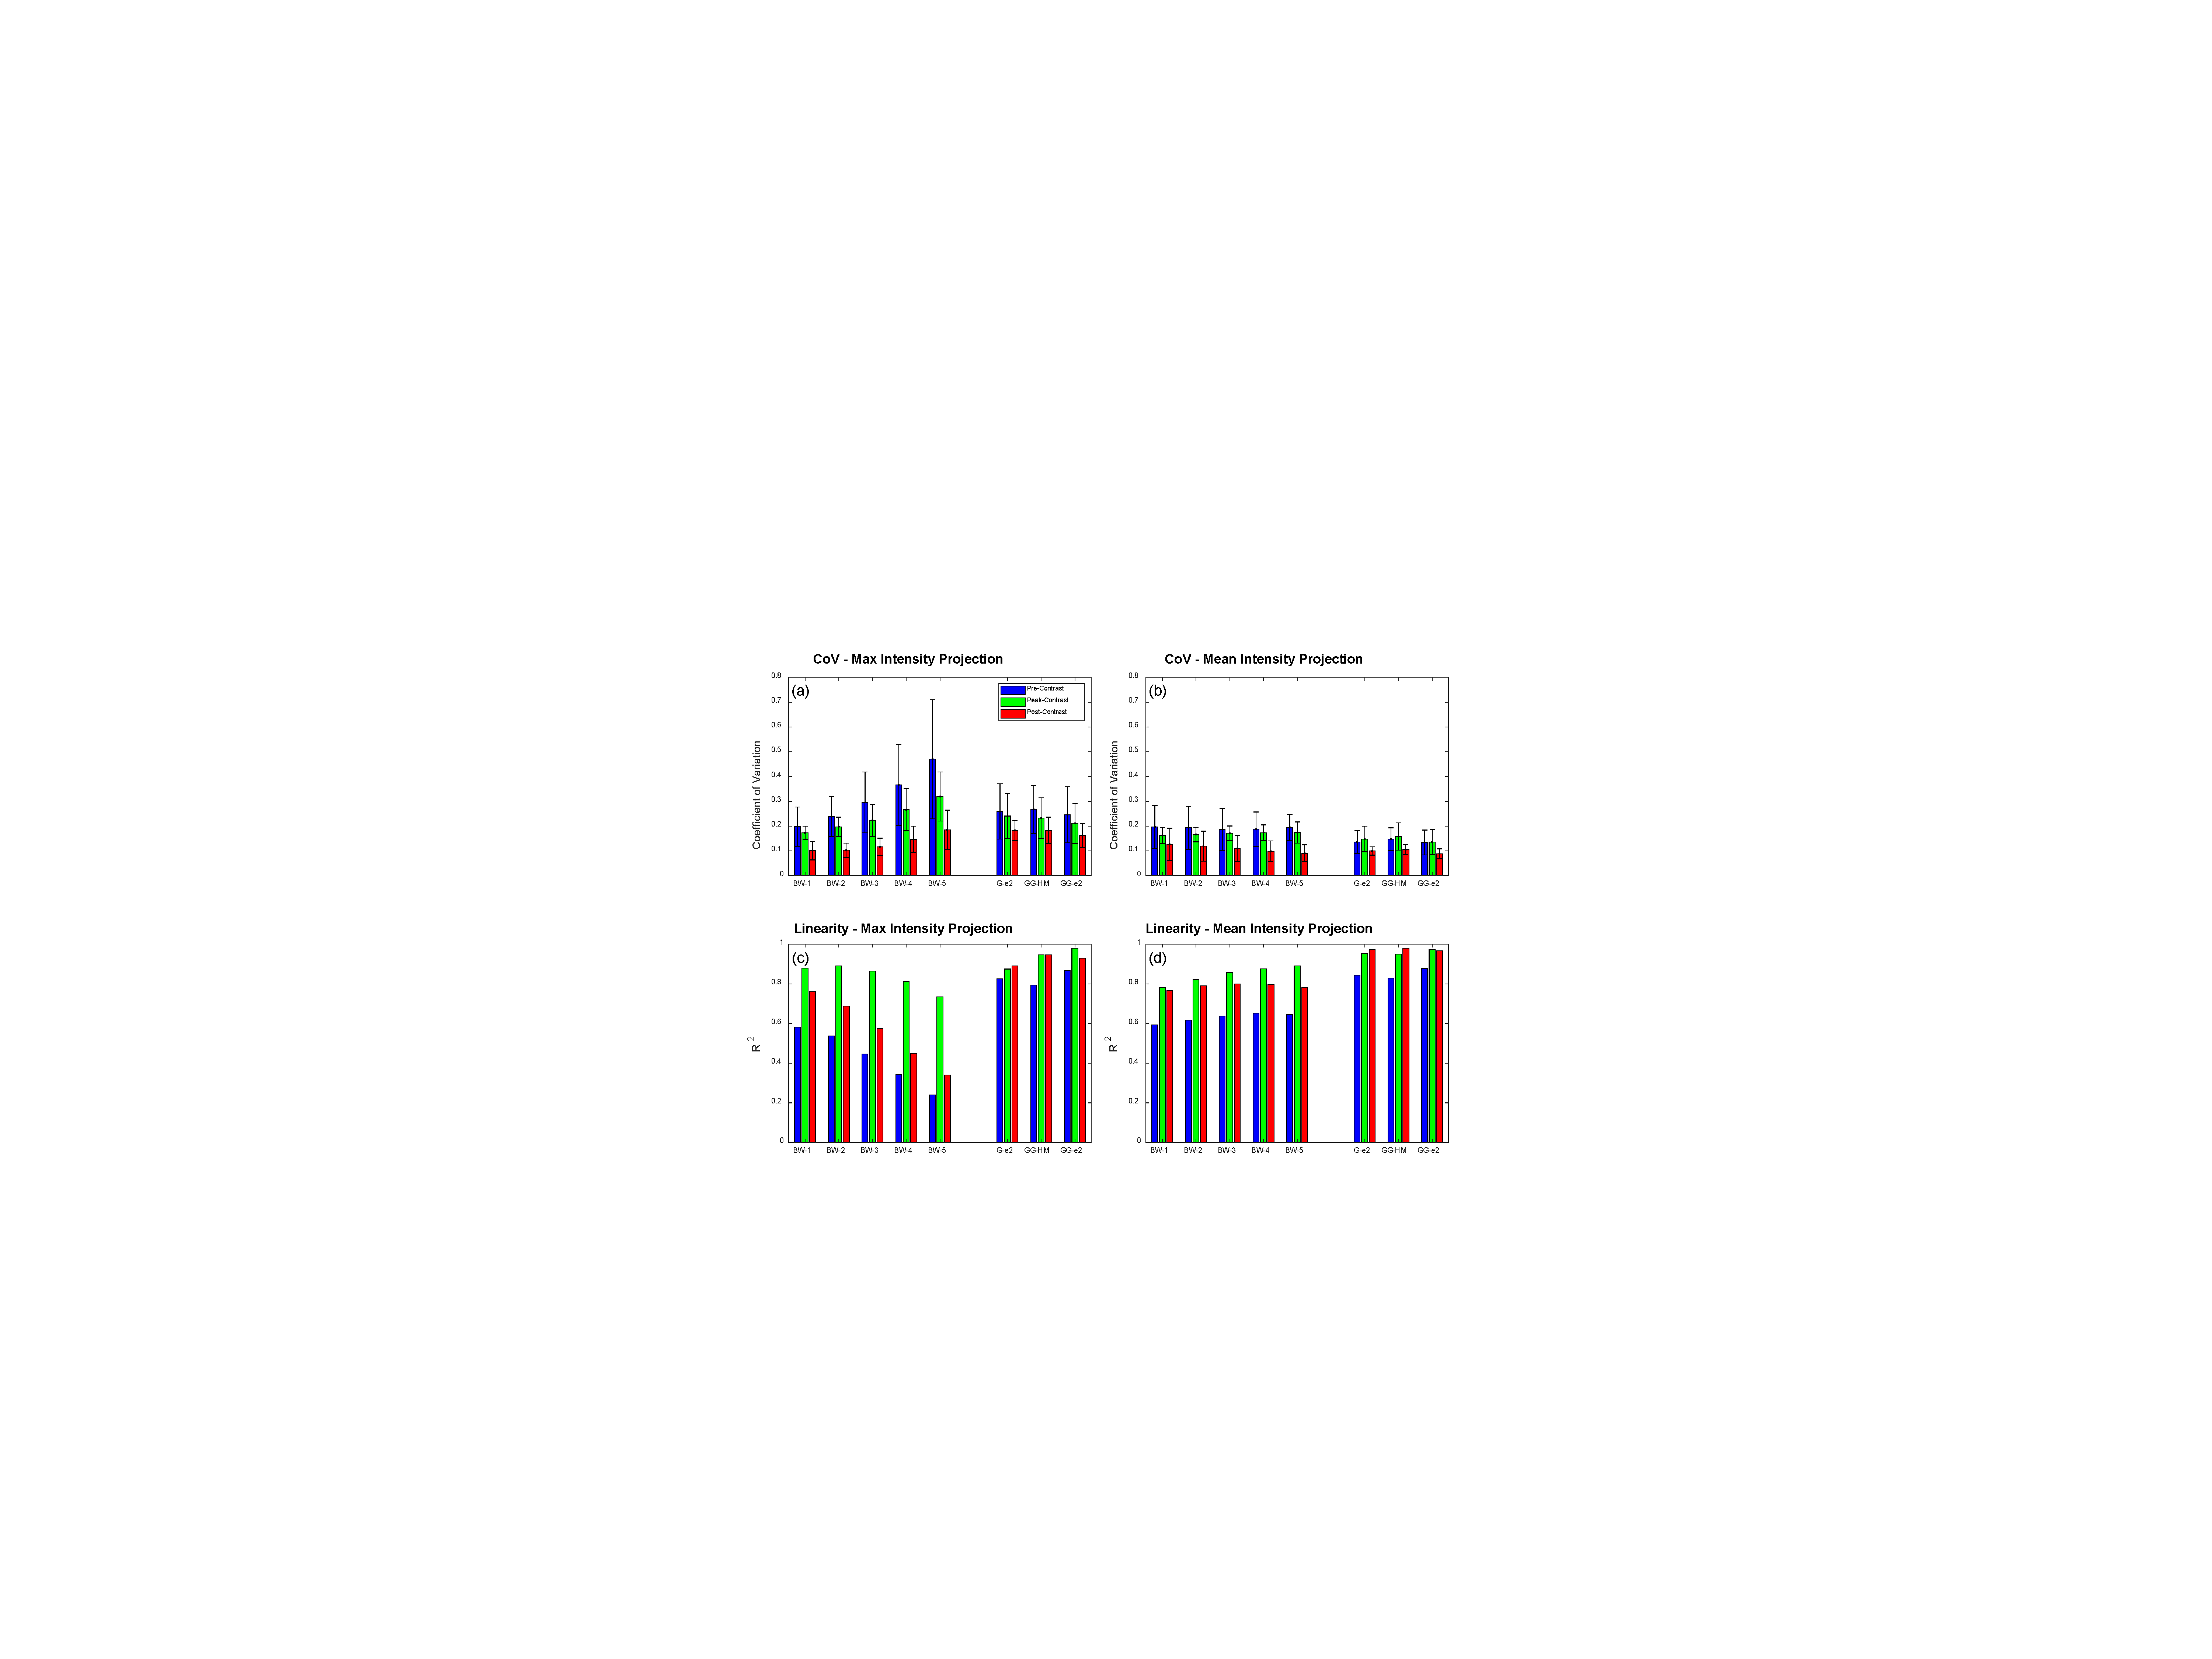
\includegraphics[width=\linewidth,height=\dimexpr\textheight-\pagetotal-10\baselineskip\relax,keepaspectratio]{figures/Figure_7.pdf}
\caption{Summary of repeatability and linearity across all diameter measurement methods. (a,b) Coefficient of variation (CoV) for MIP and MeIP, respectively. (c,d) Coefficient of determination ($R^2$) for MIP and MeIP, respectively. Bars are grouped by method (BW-1 through BW-5, G-$e^2$, GG-HM, GG-$e^2$) and colour-coded by contrast condition: pre-contrast (blue), peak-contrast (green), and post-contrast (red). Model based methods consistently show lower CoV and higher $R^2$ than binarisation based methods.}
\label{fig:cov_r2}
\end{figure}

\subsection{Functional flicker stimulation}
\label{subsec:flicker}
To investigate whether the choice of diameter measurement method affects the detection of physiological vascular responses, functional flicker stimulation was performed in a C57BL/6 mouse and vessel diameter was measured before and after photoreceptor stimulation using each of the three approaches (Fig.~\ref{fig:flicker}).

The Gaussian and GG model-based time series (Figs.~\ref{fig:flicker}a,b) showed visible diameter increases following stimulation onset for most of the five vessels examined, consistent with the expected neurovascular coupling-driven vasodilation. The binarised angiogram time series (Fig.~\ref{fig:flicker}c), however, showed the opposite trend: a paradoxical decrease in measured diameter following stimulation. Bar charts summarising the mean pre- and post-stimulation diameters per vessel (Figs.~\ref{fig:flicker}d--f) confirmed this pattern. For the Gaussian model, four of five vessels showed significant diameter increases ($p < 0.01$), with percentage changes of $+9.2\%$, $+9.6\%$, $+28.5\%$, and $+4.9\%$ for vessels 1, 2, 4, and 5, respectively (Fig.~\ref{fig:table}). The GG model similarly detected significant increases in three of five vessels ($+9.9\%$, $+28.4\%$, and $+3.1\%$ for vessels 2, 4, and 5). In marked contrast, the binarised method detected significant diameter \emph{decreases} in four of five vessels ($-12.5\%$, $-10.2\%$, $-4.2\%$, and $-9.3\%$ for vessels 1, 2, 3, and 5).

\begin{figure}[H]
\centering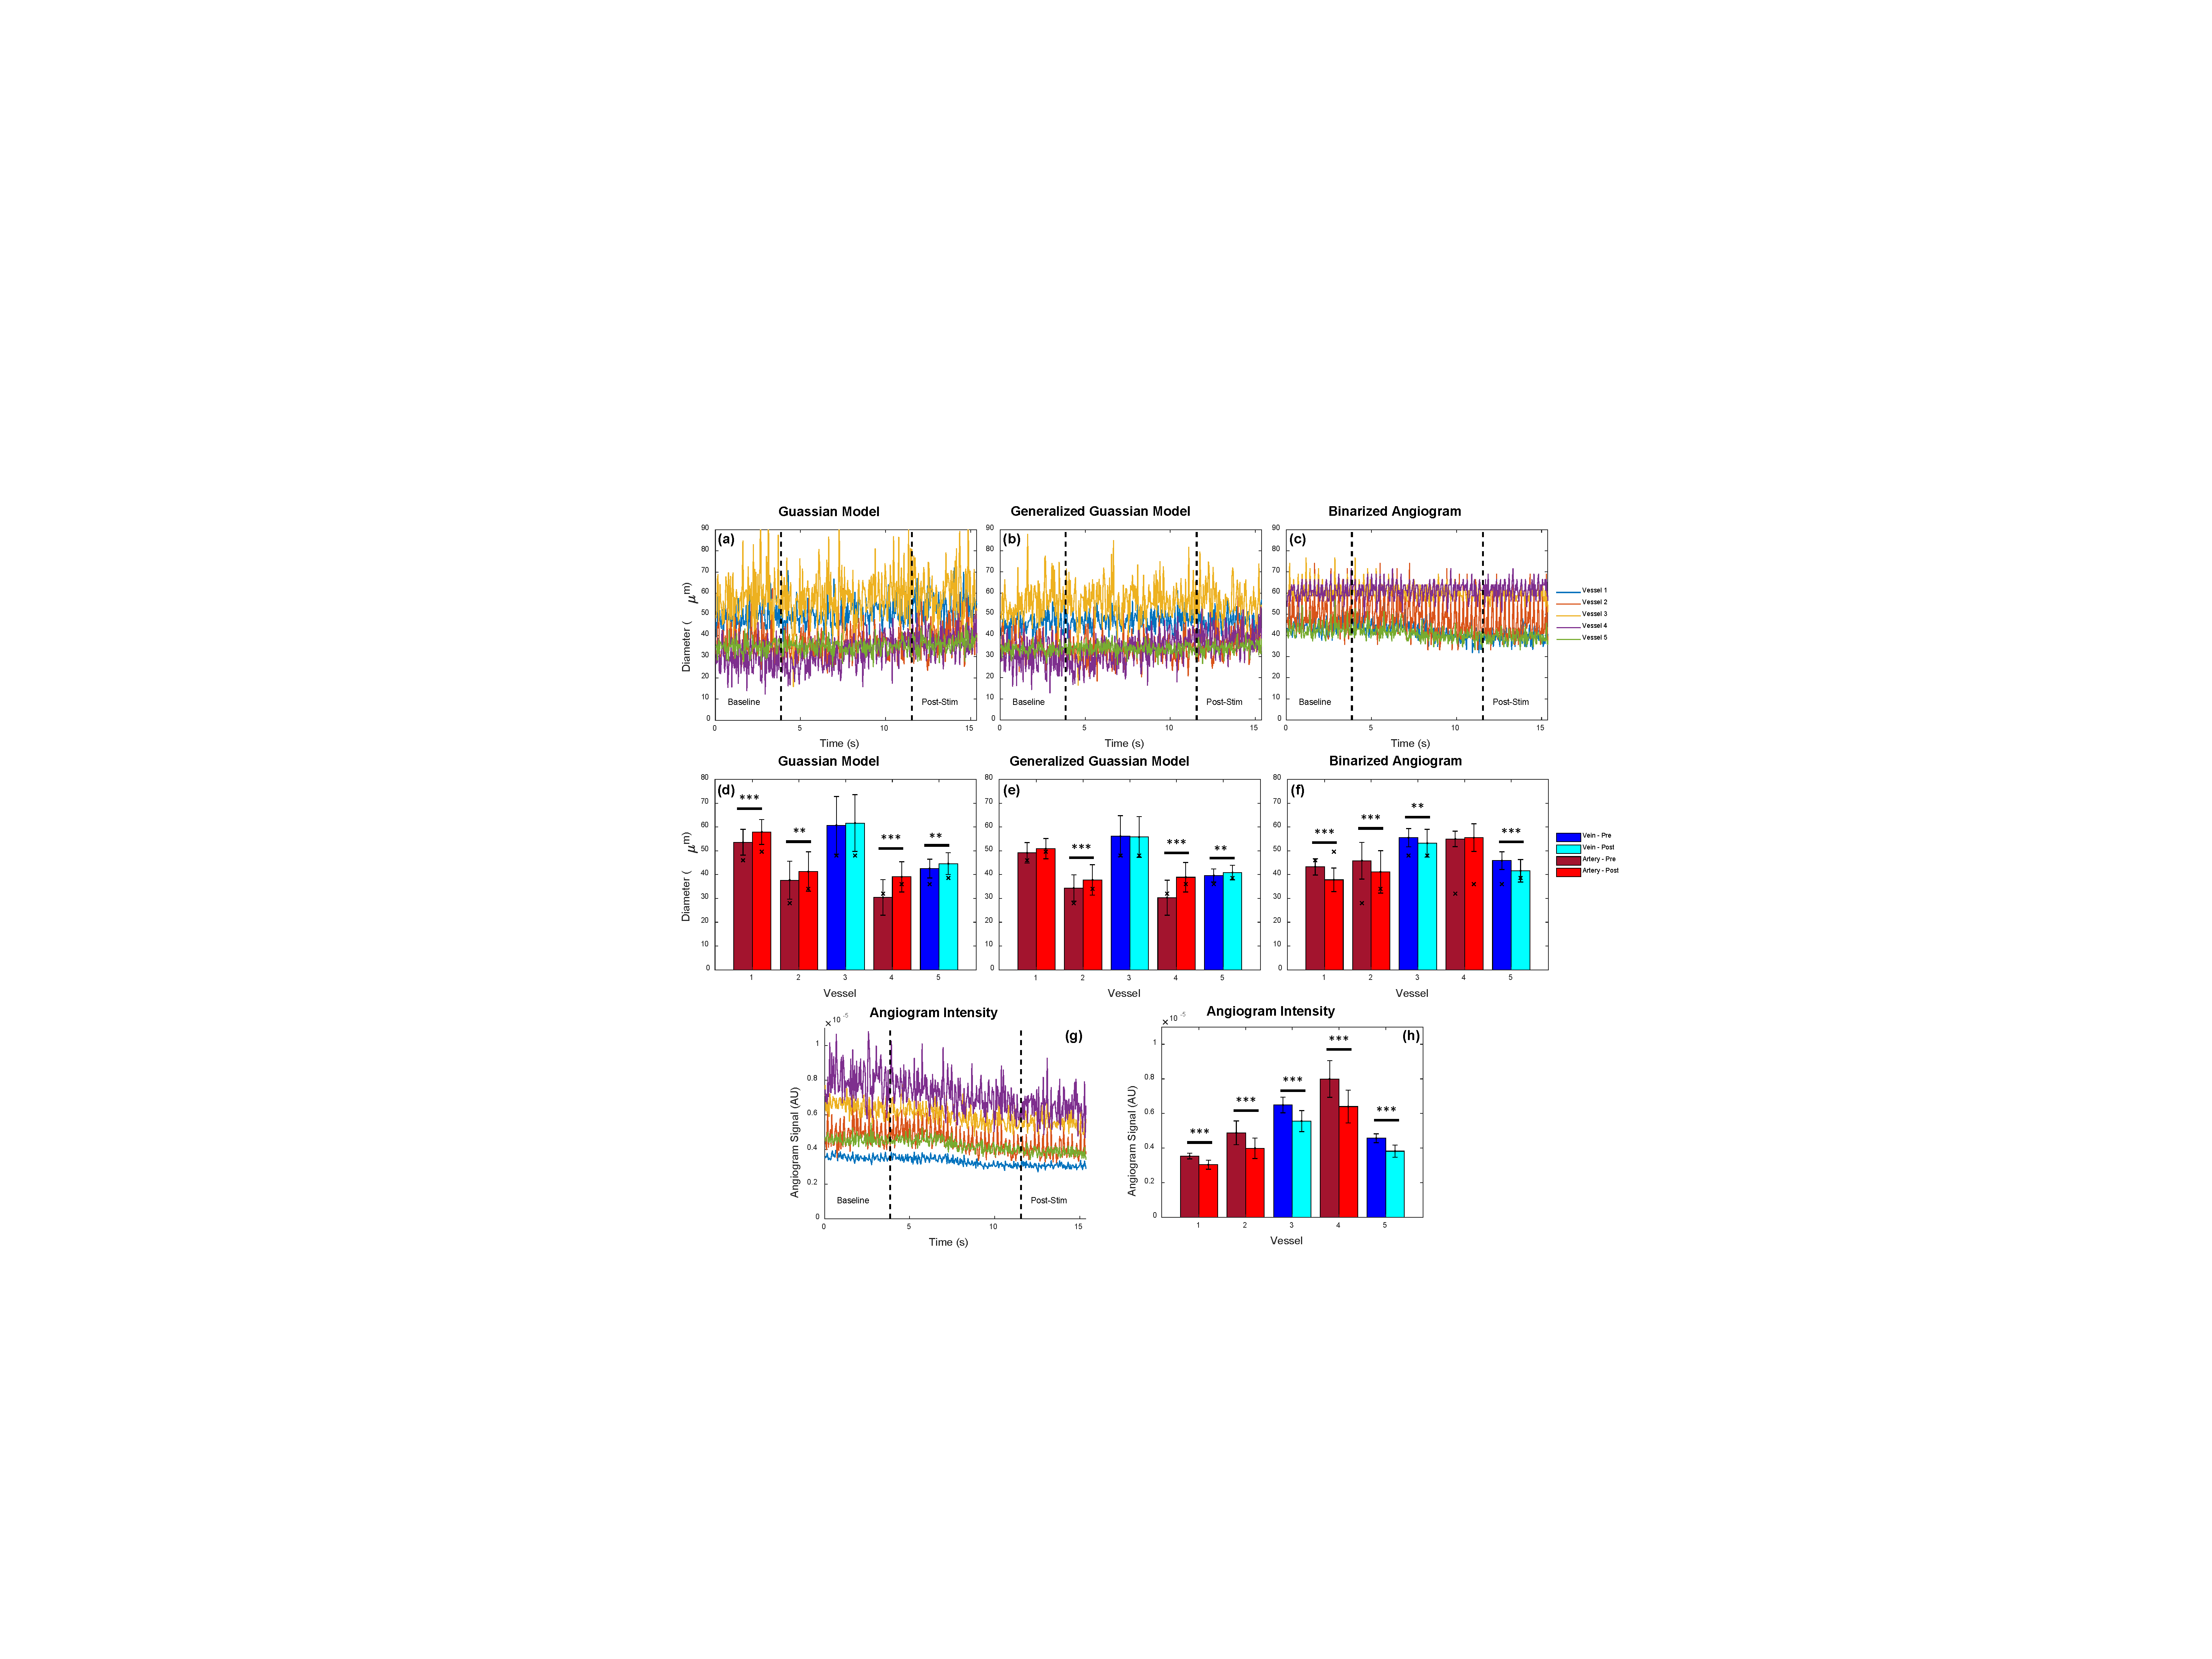
\includegraphics[width=\linewidth,height=\dimexpr\textheight-\pagetotal-14\baselineskip\relax,keepaspectratio]{figures/Figure_8.pdf}
\caption{Functional flicker stimulation results. (a--c) Time series of vessel diameter during baseline and post-stimulation periods for (a) Gaussian model, (b) generalised Gaussian model, and (c) binarised angiogram, across five vessels. Dashed lines indicate stimulation onset and offset. (d--f) Mean diameter per vessel before (dark bars) and after (light bars) stimulation for each method; veins are shown in blue/cyan and arteries in dark/light red. Significance levels: $^{**}p < 0.01$, $^{***}p < 0.001$. (g) Angiogram signal intensity time series and (h) mean intensity per vessel before and after stimulation. Model-based methods detect the expected vasodilation, whereas the binarised method paradoxically reports vasoconstriction.}
\label{fig:flicker}
\end{figure}

The explanation for this paradoxical binarisation result lies in the concomitant change in angiogram signal intensity. Following stimulation, the angiogram intensity decreased significantly for all five vessels ($p < 0.0005$), with reductions ranging from $-14.1\%$ to $-19.9\%$ (Figs.~\ref{fig:flicker}g,h; Fig.~\ref{fig:table}). Because the binarised diameter is derived from the number of pixels exceeding a fixed threshold, a reduction in signal intensity directly translates to fewer above-threshold pixels and hence a smaller apparent diameter, even if the true vessel diameter has increased.

To quantify this confounding, the correlation between diameter change and angiogram intensity change was computed for each method (Table~\ref{fig:table}). For the binarised method, the per-vessel correlations were uniformly positive and strong ($\rho = 0.59$, $0.80$, $0.27$, $0.46$, $0.52$ for vessels 1--5), yielding an overall correlation of $\rho = 0.523$ ($p < 0.0005$). This indicates that the binarised diameter measurement is substantially confounded by the angiogram signal intensity. In contrast, the Gaussian model yielded an overall correlation of $\rho = -0.101$ and the GG model yielded $\rho = -0.098$, confirming that the model-based diameter measurements are effectively independent of angiogram signal intensity fluctuations. These results demonstrate that model-based fitting not only provides more accurate and repeatable diameter measurements, but also recovers physiologically meaningful vascular responses that binarisation-based methods can misrepresent.

\begin{table}[htbp]
\caption{Summary of flicker stimulation results. Top: percentage diameter change per vessel for each method together with corresponding $p$-values. Bottom: Pearson correlation ($\rho$) between measured diameter and angiogram signal intensity for each method and vessel. Overall correlations: Gaussian $= -0.101$, GG $= -0.098$, BW $= 0.523$.}
\label{fig:table}
\centering
\resizebox{\textwidth}{!}{%
\begin{tabular}{l c c c c c c c c c c}
\hline
\textbf{Change in Diameter} & \multicolumn{2}{c}{\textbf{Vessel 1}} & \multicolumn{2}{c}{\textbf{Vessel 2}} & \multicolumn{2}{c}{\textbf{Vessel 3}} & \multicolumn{2}{c}{\textbf{Vessel 4}} & \multicolumn{2}{c}{\textbf{Vessel 5}} \\
\hline
Gaussian (\% Change) & \textbf{9.2} & $p < 0.0005$ & \textbf{9.6} & $p = 0.0019$ & 1.5 & $p = 0.59$ & \textbf{28.5} & $p < 0.0005$ & \textbf{4.9} & $p = 0.0008$ \\
Gen.\ Gaussian (\% Change) & 1.5 & $p = 0.28$ & \textbf{9.9} & $p < 0.0005$ & $-0.6$ & $p = 0.79$ & \textbf{28.4} & $p < 0.0005$ & \textbf{3.1} & $p = 0.0034$ \\
Binarised (\% Change) & $\mathbf{-12.5}$ & $p < 0.0005$ & $\mathbf{-10.2}$ & $p < 0.0005$ & $\mathbf{-4.2}$ & $p = 0.0011$ & 1.0 & $p = 0.404$ & $\mathbf{-9.3}$ & $p < 0.0005$ \\
Angiogram Intensity (\% Change) & $\mathbf{-14.1}$ & $p < 0.0005$ & $\mathbf{-18.2}$ & $p < 0.0005$ & $\mathbf{-14.3}$ & $p < 0.0005$ & $\mathbf{-19.9}$ & $p < 0.0005$ & $\mathbf{-16.3}$ & $p < 0.0005$ \\
\hline
\\[-0.5em]
\hline
\textbf{Correlation to Intensity} & \multicolumn{2}{c}{\textbf{Vessel 1}} & \multicolumn{2}{c}{\textbf{Vessel 2}} & \multicolumn{2}{c}{\textbf{Vessel 3}} & \multicolumn{2}{c}{\textbf{Vessel 4}} & \multicolumn{2}{c}{\textbf{Vessel 5}} \\
\hline
Gaussian Diameter Corr.\ & $-0.07$ & $p = 0.48$ & \textbf{0.23} & $p = 0.019$ & $\mathbf{-0.28}$ & $p = 0.0044$ & $-0.15$ & $p = 0.14$ & $\mathbf{-0.24}$ & $p = 0.018$ \\
Gen.\ Gaussian Diameter Corr.\ & 0.03 & $p = 0.79$ & 0.07 & $p = 0.47$ & $\mathbf{-0.28}$ & $p = 0.0056$ & $-0.14$ & $p = 0.16$ & $-0.18$ & $p = 0.081$ \\
Binarised Diameter Corr.\ & \textbf{0.59} & $p < 0.0005$ & \textbf{0.80} & $p < 0.0005$ & \textbf{0.27} & $p = 0.0077$ & \textbf{0.46} & $p < 0.0005$ & \textbf{0.52} & $p < 0.0005$ \\
\hline
\end{tabular}%
}
\end{table}
% ~\FloatBarrier~%print all pending figures/tables right here, don’t let them move past this point.

\section{Discussion}
 % Discussion

\subsection{Model-based vs binary mask based diameter measurement}
\label{subsec:model_vs_binary}
The model-based and binary mask based diameter methods define vessel boundary in fundamentally different ways. Binarisation of the en face maps discards the spatial intensity distribution for a simple binarisation and reduces each pixel to a binary decision. The measured diameter directly depends on the chosen threshold value and on angiogram intensity, both of which may vary across imaging sessions, contrast conditions, and even between vessels within the same scan. Model-based methods fit a parametric model function to the maximum or mean intensity profiles, and calculate the diameter from the fitted parameters. As the fit captures the shape of the profile rather than the absolute intensity, it is inherently less sensitive to changes in angiogram signal and does not require a threshold at all.

A practical consequence of this difference is how correctable each method is. Because the model-based fit requires no threshold, it returns a single consistent value for a given profile, whereas the binarisation slope shifts with the chosen threshold, so any calibration must also encode which threshold was used. Underestimation can be corrected by a fixed proportion using the slope, provided the relationship with the ground truth is strongly linear, but such a rescaling removes only the systematic offset and leaves the scatter about the regression unchanged. Linearity, rather than slope alone, therefore determines how reliably a method can be corrected. Post-contrast every model-based metric reached $R^2 \geq 0.92$, whereas binary mask based MIP fell from 0.81 at BW-1 to 0.48 at BW-5, so more than half the variance would remain after any correction. This is what makes the higher-linearity model-based metrics usable even pre-contrast, where $w_{1/e^2,\mathrm{GG}}$ retained $R^2 = 0.81$ against 0.62 for the best binary mask based method.

This difference explains the trends observed in Fig.~\ref{fig:cov_r2} and Table~\ref{tab:accuracy_linearity}. Post-contrast, every model-based metric was more linear than every binary mask based method, and the GG $1/e^2$ metric reached near-unity slopes at peak and post-contrast without a threshold parameter to tune, whereas for the binary mask based methods linearity was overall lower and depended on threshold. Because the peak angiogram intensity varies between vessels, a fixed threshold removes a different fraction of the cross-section from each one. The measured diameters therefore vary from the ground truth by different amounts, which weakens the linearity. Pre-contrast, the hourglass artefact caused by RBC orientation within vessel lumen suppresses edge signals, causing all methods to underestimate diameter~\cite{bernucciInvestigationArtifactsRetinal2018}. However, model-based methods still retained more of that linearity, producing systematic, predictable underestimation. Binary mask based methods on the other hand showed weaker linearity in most conditions, potentially because the suppressed edge signals did not consistently exceed the binarisation threshold, and because different vessels have different intensity.

The same mechanism accounts for how each method responded to the change in angiogram intensity from peak to post-contrast. Angiogram intensity is highest as the bolus arrives and then settles to a lower steady state (Fig.~\ref{fig:dycoct}f), so a fixed threshold encloses a smaller fraction of each cross-section post-contrast than at peak, an effect visible in the binarised cross-sections over time (Fig.~\ref{fig:dycoct}d,e). Model-based metrics were largely insensitive to this, changing by at most 0.04 in slope and 0.04 in $R^2$ between the two conditions. Binary mask based measurements from MIP degraded progressively with threshold, the slope falling by 0.04 at BW-1 but 0.11 at BW-5, and $R^2$ by 0.07 and 0.30 respectively, while MeIP remained comparatively stable (slope change 0.02--0.03 at every threshold). Model-based methods therefore showed comparable agreement with the ground truth at both peak and post-contrast, whereas the agreement of binarisation depended on the combination of threshold and contrast condition.

The generalised Gaussian (GG) model will always outperform the standard Gaussian because the intensity profiles of the vessels are usually not purely Gaussian (Fig.~\ref{fig:gg_model}b). The standard Gaussian cannot capture relatively flat-topped angiogram intensity profiles and tends to fit a narrower curve, whereas the GG model accommodates through the shape parameter $\beta$, which ranges from Gaussian ($\beta = 2$) to increasingly flat-topped profiles ($\beta > 2$). The flat-topped shapes arise because the measured profile is effectively the vessel's reflectivity profile convolved with the system point spread function. Because the GG reduces to a standard Gaussian when $\beta = 2$ and departs from it only when the data support a flatter profile, a correctly applied GG fit should perform at least as well as the Gaussian, at the cost of additional computation.

Among the width metrics, $w_{fwhm,\,\mathrm{GG}}$ consistently showed the weakest accuracy, although its linearity remained high post-contrast ($R^2$ = 0.96 for MIP and 0.98 for MeIP), indicating that the underestimation is systematic and therefore correctable. Near the half-maximum the profile shape changes rapidly and varies between vessels, from Gaussian to flat-topped, so the width measured at that level is more variable. The $1/e^2$ width captures more of the transition region and so may have provided a more accurate measurement of the vessel diameter.

\subsection{Maximum vs mean intensity projection}
\label{subsec:max_vs_mean}
Across nearly all methods and conditions, MeIP outperformed MIP in both accuracy and precision (Table~\ref{tab:accuracy_linearity}). Linearity was the exception. Pre-contrast MIP produced higher $R^2$ than MeIP for all model-based metrics, and MIP also produced higher $R^2$ at the two lowest binarisation thresholds, with MeIP outperforming MIP only post-contrast.  This finding is noteworthy because MIP has been shown to produce higher signal-to-noise ratio (SNR) and contrast in en face OCTA images~\cite{hormelMaximumValueProjection2018}, and is the default in many commercial OCTA systems and analysis pipelines~\cite{sampsonTowardsStandardizingRetinal2022,untrachtTowardsStandardisingRetinal2024}. However, we observed that higher SNR did not necessarily translate to more accurate diameter measurements. The MIP selects the single highest intensity value along each A-scan within the vessel ROI, which makes it inherently sensitive to outliers. MeIP averages all intensity values along each A-scan, which smooths out intensity fluctuations and provides a consistent profile. This averaging could be beneficial for vessel diameter measurement, as the goal is to capture the typical vessel boundary rather than extreme signal events. This trade-off may also explain why linearity behaved differently before and after contrast. Pre-contrast the vessel signal is weakest, and edge suppression by the RBC orientation artefact leaves little margin above the background, so the higher contrast of the MIP helps keep the profile distinguishable across vessels of different size. Once the lumen is filled with contrast agent, signal is no longer limiting and the outlier sensitivity of a maximum statistic becomes the dominant source of error, so the averaging of the MeIP yields the tighter relationship with the ground truth. Consistent with this, MeIP produced higher $R^2$ than MIP for all three model-based metrics post-contrast, whereas at peak contrast the two projections remained comparable, with MIP higher for two of the three.

The difference between MIP and MeIP was especially apparent in the binary mask based results (Table~\ref{tab:accuracy_linearity}). For MeIP, the slope declined more gradually and remained at 0.86 even at BW-5 post-contrast. Whereas for MIP, the slope decreased steeply with increasing threshold, dropping from 0.92 at BW-1 to 0.54 at BW-5 post-contrast. These findings suggest that MeIP produces a more uniform intensity distribution across the vessel profile, making the binarisation result less sensitive to the exact threshold value. The CoV data (Table~\ref{tab:accuracy_linearity}) reinforced this as the MIP-based binary mask CoV increased substantially with threshold, whereas the MeIP-based CoV remained relatively stable. This behaviour follows from how each projection responds to variance in the angiogram signal. The MIP retains only the brightest pixel along each A-scan, so it is a maximum statistic and follows the largest excursion in the signal, and the projected profile therefore varies from one time sample to the next. A fixed threshold applied to a varying profile returns a varying width, and the higher the threshold the nearer the peak that width is measured, where a given change in intensity displaces the threshold crossing further. The CoV consequently grows with threshold. MeIP instead averages along each A-scan, which suppresses this variance and produces a broader, smoother profile, leaving the CoV largely unchanged as the threshold increases. For model-based methods, MeIP also showed better performance. The $w_{1/e^2,\,\mathrm{G}}$ using MIP slightly overestimated vessel diameter post-contrast with $m = 1.12$, while MeIP reduced this to $m = 1.04$, a much closer agreement with the ground truth. These results suggest that while MIP may be preferred for visualisation purposes where contrast and SNR are important~\cite{hormelMaximumValueProjection2018}, MeIP should be the preferred projection method for quantitative diameter measurements.

\subsection{Influence of angiogram intensity on diameter measurements}
\label{subsec:influence_of_intensity}
The functional flicker stimulation experiment provided a direct demonstration of how changes in angiogram signal intensity can affect diameter measurements based on the method used. During the DyC-OCT acquisition, the angiogram intensity declined significantly across all five vessels (Fig.~\ref{fig:flicker}g,h), with decreases ranging from $-13.6\%$ to $-19.8\%$ (Table~\ref{tab:flicker}). The cause of this decline was not established with certainty, although inspection of the volumetric data ruled out the most important confounds. There was no out-of-plane motion or breathing artefact, and the image quality was consistent throughout the scan. We suspect a combination of rapid corneal drying and/or cataract formation over the course of the scan could have caused the decline in intensity. More importantly, the cause of the decline is not essential to our argument for this study, what matters is that the intensity decline biases the binary mask based diameter measurement while the model-based diameter remains unaffected. 

The model-based methods correctly detected the expected vasodilation, with the Gaussian model showing significant diameter increases in four of five vessels ($+15.5\%$ overall in the arteries against $+3.1\%$ in the veins) and the GG model showing significant increases in four of five vessels ($+14.0\%$ and $+1.4\%$ respectively; Table~\ref{tab:flicker}). The binary mask based method, however, reported significant diameter decreases in four of five vessels, suggesting vasoconstriction which is a paradoxical result. The reason behind this behaviour could be understood by observing how each method responds to declining signal intensity (Fig.~\ref{fig:scatter_intensity}). For the binary mask based method, the threshold is fixed and diameter is determined by the number of pixels that exceed this threshold. When the overall angiogram intensity drops, fewer pixels at the vessel edges exceed the threshold, and the vessel appears to shrink even if the physical vessel diameter has increased. This is confirmed by the strong positive correlation between measured diameter and angiogram intensity for the binary mask based method ($\rho = 0.526$, $p < 0.0005$). In contrast, the model-based methods showed weak overall correlations with intensity ($\rho = -0.101$ for Gaussian, $\rho = -0.098$ for GG), indicating that the fitted diameter was effectively independent of the signal intensity. Among the methods, the GG model also produced the lowest standard deviations across the five vessels in the flicker experiment (Fig.~\ref{fig:flicker}d--f), consistent with its low CoV post-contrast (Table~\ref{tab:accuracy_linearity}), indicating that it is the most repeatable of the metrics tested. Together these results demonstrated that the model-based diameter calculation provided more accurate and repeatable measurements, and recovered physiologically meaningful vascular responses that binary mask based methods misrepresented.

These findings have important implications for longitudinal studies and any experiment where angiogram intensity may vary between or within imaging sessions. In longitudinal mouse eye imaging, the angiogram signal can vary between and within sessions as anaesthesia alters retinal perfusion and ocular physiology~\cite{wormRetinalOCTParameters2026,fengHighresolutionStructuralFunctional2023}, with additional factors such as cataract formation, and corneal drying if tear drops are not applied, further reducing OCT intensity over time~\cite{steinEffectCornealDrying2006,mclellanOpticalCoherenceTomography2012}. If a binary mask based method is used under such conditions, observed changes in vessel diameter may reflect intensity fluctuations rather than true vascular changes. In contrast, model-based methods may be less sensitive to these intensity variations, as they characterise the shape of the intensity profile rather than relying primarily on absolute intensity values to define vessel boundaries.

\subsection{Threshold selection}
\label{subsec:threshold_selection}
The results presented here used a basic, global threshold for the binarisation of the angiogram data. There are numerous other approaches for binarising the angiogram, which will most likely each behave differently. For example, angiogram signals can be enhanced with vesselness filters~\cite{frangiMultiscaleVesselEnhancement1998} and dynamic thresholds can be used to binarise images with varying SNR. When applying a vesselness filter, it is possible to enhance the shape of the angiogram and omit noise, but it is also possible for such enhancement to overcompensate the signal, leading to larger than expected vessel appearance. Measurements obtained with different enhancement filters have been shown to differ substantially and are not interchangeable~\cite{hongEffectVesselEnhancement2020}. Dynamic thresholding can also yield a more uniform angiogram appearance, but similarly risks over- or under-compensating vessels. The threshold chosen is known to alter OCTA quantitative metrics systematically, with automatic thresholds tending to underestimate relative to a fixed threshold~\cite{mehtaImpactBinarizationThresholding2019,arrigoImpactDifferentThresholds2021}. Further analysis of these other methods would be required to determine their efficacy in returning accurate and precise diameter values.

The key observation from the present work is that any thresholding approach, regardless of how the threshold is determined, shares the same fundamental limitation that the measured diameter depends on the absolute signal intensity at the vessel edges. As demonstrated by the flicker stimulation experiment, this intensity dependence can introduce artefactual diameter changes when the angiogram signal varies over time or between sessions. A more adaptive thresholding strategy may reduce variability across different regions of a single image, but it would not eliminate the sensitivity to temporal intensity fluctuations that we observed. The model-based approach avoids this limitation entirely by deriving diameter from the shape of the intensity profile rather than from an intensity cut-off, making it a fundamentally different and more robust alternative for quantitative diameter analysis.

\subsection{Best choices under different conditions}
\label{subsec:best_choices}
Under the conditions where a contrast agent is available and accuracy is the primary goal, the $w_{1/e^2,\,\mathrm{GG}}$ metric using MeIP provides the best results post-contrast. This combination achieved a slope of $m = 1.001$ with $R^2 = 0.97$ and a CoV of 0.09, yielding the best accuracy, linearity, and precision of all tested methods. If only pre-contrast data is available, the $w_{1/e^2,\,\mathrm{GG}}$ metric still provides the best linearity among all tested methods ($R^2 = 0.81$ for MIP, $R^2 = 0.76$ for MeIP), though the MIP and MeIP slope of $m = 0.64$ and $m = 0.71$ indicates that diameter could be underestimated by approximately 35\% and 30\% respectively. In this case, a correction factor could be applied if absolute diameter values are needed, though relative comparisons between vessels or timepoints would remain valid without correction.

When only MIP data is available, which is the case for many commercial OCTA machines and existing datasets~\cite{sampsonTowardsStandardizingRetinal2022,untrachtTowardsStandardisingRetinal2024}, the $w_{1/e^2,\,\mathrm{GG}}$ still provides good post-contrast accuracy ($m = 1.02$, $R^2 = 0.95$). For binary mask based analysis of MIP data, only the lowest threshold (BW-1) post-contrast achieved a slope near unity ($m = 0.92$), and the slope degraded rapidly with increasing threshold values. This highlights that if binarisation must be used with MIP data, a lower threshold value is essential, though this may come at the cost of increased noise sensitivity.

The improved linearity and repeatability of the model-based approaches come at the cost of computation time, as fitting a model is considerably more expensive than binarisation. In our testing, fitting the generalised Gaussian was approximately 40\% slower than the standard Gaussian. This difference is hardware dependent, and because the fits at each cross-section are independent, the computation could be parallelised and accelerated with appropriate hardware. If computation time is a limiting factor and model fitting is not practical, MeIP with a moderate threshold (e.g.\ BW-3) provides a reasonable alternative. At post-contrast, BW-3 using MeIP achieved $m = 0.96$ and $R^2 = 0.81$, which is acceptable for many applications. MeIP-based binary mask based analysis showed more stable CoV values across all thresholds compared to MIP, making the results less sensitive to the exact threshold choice. This stability makes MeIP the preferred projection for binary mask based OCTA.

\subsection{Literature comparison}
\label{subsec:literature_comparison}

Hormel et~al.~\cite{hormelMaximumValueProjection2018} showed that MIP produces en face OCTA images with higher SNR and contrast compared to MeIP, and concluded that MIP should be preferred for OCTA visualisation. Our results reveal a different picture when it comes to quantitative vessel diameter measurement. We found that MeIP consistently yielded more accurate and precise diameter values than MIP across both model-based and binary mask based approaches, with the exception of pre-contrast linearity, where MIP performed better. This suggests that the projection method best suited for visualisation is not necessarily the best suited for quantification, and that the choice of projection should depend on the intended analysis.

The challenge of standardising OCTA image analysis has been highlighted by Sampson et~al.~\cite{sampsonTowardsStandardizingRetinal2022} and Untracht et~al.~\cite{untrachtTowardsStandardisingRetinal2024}, both of whom emphasised the need for transparent, reproducible analysis pipelines. Our findings add to this discussion by showing that the choice of diameter measurement method introduces a source of variability that is at least as significant as the choice of binarisation threshold. The model-based approach presented here offers a path toward more standardised vessel diameter quantification, as it reduces the dependence on selected thresholds and angiogram intensity, and provides measurements that are more robust across imaging conditions.

The RBC orientation artefact and its effect on OCTA vessel appearance has been described by Cimalla et al.~\cite{cimallaShearFlowinducedOptical2011} and Bernucci et~al.~\cite{bernucciInvestigationArtifactsRetinal2018}, who used Intralipid contrast to demonstrate that the hourglass pattern in vessel cross-sections is caused by the directional scattering properties of RBCs rather than by true variations in flow. Our work extends this observation by quantifying the degree to which this artefact affects diameter measurements and by proposing model-based fitting as a practical correction strategy. While contrast enhancement with Intralipid is effective for revealing the true vessel diameter, it requires a contrast injection and is not yet applicable in clinical settings. Using a calibrated model-based approach provides a way to partially recover the underestimated diameter from native OCTA data without the need for a contrast agent.

Recent work by Son et~al.~\cite{sonFunctionalOCTReveals2024} used functional OCT to image flicker-evoked vasodilation in the mouse retina and reported that vasodilation is anisotropic, with larger percent changes in the axial direction ($\sim18\%$) than the lateral direction ($\sim11\%$). The authors did not describe how vessel diameters were quantified from their B-scans. It is worth considering whether the lateral diameter measurements may have been affected by the intensity-dependent artefacts observed in the present work. In the lateral direction, the RBC orientation artefact suppresses signal at vessel edges, and depending on how their vessel boundary was defined, this artefact could lead to an underestimation of the lateral diameter. If this were the case, the apparent difference between axial and lateral vasodilation could be influenced by the measurement methodology in addition to the biomechanical anisotropy discussed by the authors. It would be interesting to apply the model-based approach presented here to such data to determine whether their reported anisotropy changes when the lateral diameter is quantified differently.

The magnitude of vasodilation detected by the generalised Gaussian model ranged from $+3.1\%$ to $+28.4\%$ across the vessels with a significant response (Table~\ref{tab:flicker}). The arteries (Vessels 1, 2, and 4) showed increases of $+3.5\%$, $+10.1\%$, and $+28.4\%$, while the veins (Vessels 3 and 5) showed a smaller response, with $+3.1\%$ in Vessel 5 and no significant change in Vessel 3. The standard Gaussian gave a broadly similar picture, with arterial increases of $+8.2\%$, $+9.9\%$, and $+28.5\%$ and a venous increase of $+4.9\%$ in Vessel 5. Table~\ref{tab:flicker_comparison} summarises the stimulation protocols and vascular responses reported by previous flicker stimulation studies alongside our own. The listed human studies span several measurement techniques, from fundus photography~\cite{formazDiffuseLuminanceFlicker1997} through retinal vessel analysers~\cite{polakInfluenceFlickerFrequency2002,garhoferDiffuseLuminanceFlicker2004,nagelFlickerObservationLight2004} to Doppler OCT~\cite{aschingerEffectofDiffuse2017} and OCTA~\cite{kallabPlexusSpecificEffect2020}. Despite these methodological differences, the reported human arterial responses cluster between $+3\%$ and $+8\%$, and venous responses between $+2\%$ and $+10\%$. Notably, these studies report arterial and venous responses of broadly comparable magnitude, and in some cases the venous response is the larger of the two, for example $+9.8\%$ venous versus $+8.0\%$ arterial in Aschinger et~al.~\cite{aschingerEffectofDiffuse2017}. This contrasts with our measurements, in which the arterial response was on average larger than the venous response. Whether this asymmetry reflects a genuine feature of the murine flicker response, the small number of vessels sampled, or a greater sensitivity of the model-based fit to the smooth-muscle-driven dilation of arteries remains to be established. Polak et~al.~\cite{polakInfluenceFlickerFrequency2002} additionally showed that the diameter response is relatively stable across flicker frequencies from 4 to 40~Hz, suggesting that frequency differences between studies are unlikely to explain the variation.

The magnitudes we observed are generally larger than those reported in the human studies, though direct comparison is difficult given the differences in experimental conditions. Species, anaesthesia, stimulation frequency and wavelength, stimulus power and delivery method, stimulation duration, dark adaptation period, and imaging modality all vary across the reported studies, and each of these factors could influence the measured vascular response. Among the studies listed, Son et~al.~\cite{sonFunctionalOCTReveals2024} used the most similar setup to ours. They used the same mouse strain (C57BL/6J), the same anaesthetic (ketamine/xylazine), a comparable flicker stimulus (10~Hz, 504~nm), however a different stimulation period of 5~s. Because the diameters reported here are lateral, their lateral values offer the closest comparison: they reported $+10.8\%$ in the arteries and $+8.9\%$ in the veins, against $+14.0\%$ and $+1.4\%$ respectively for the GG model in this study. The arterial responses are therefore of comparable magnitude, whereas our venous response is substantially smaller. A systematic comparison of these parameters could help determine which factors are most influential to the results observed in both studies. Importantly, regardless of the absolute magnitude, the fact that we were able to detect vasodilation at all depended on the measurement method, because binary mask based analysis not only failed to detect vasodilation but reported vasoconstriction which would have led to fundamentally incorrect physiological conclusions.

Previous studies in mice have measured flicker-evoked retinal vessel diameter changes mostly using dynamic vessel analysis (DVA), which is a fundus camera-based technique adapted from human retinal vessel analysers. Albanna et~al.~\cite{albannaNonInvasiveEvaluation2018} demonstrated the feasibility of DVA in the mouse eye using 12.5~Hz flicker at 530~nm but found that quantitative arterial recordings were possible only in a minority of animals, while venous dilation was mostly below 1.5\% post-stimulation. Another study by Neumaier et~al.~\cite{neumaierEvaluationFlickerInduced2021} used the same setup in wildtype and Cav2.3-deficient mice with overnight dark adaptation and reported median arterial and venous diameter changes of only $+1.3\%$ and $+1.2\%$, respectively, in the wildtype group. These values are substantially smaller than those we observed, which could be due to the limited spatial resolution and signal-to-noise ratio of DVA when applied to the smaller mouse eye rather than being a genuine physiological response. The much larger responses we observed may therefore partly result from the higher lateral resolution of OCT combined with the model-based fitting approach, which captures vessel boundary shifts that could fall below the detection limit of DVA. In addition to these diameter-based studies, Rai et~al.~\cite{raiEffectsFlickeringLight2025} recently reported that 12~Hz flicker stimulation significantly increased both arterial and venous retinal blood flow in light-adapted C57BL/6J mice. An earlier OCT-based study by Radhakrishnan and Srinivasan~\cite{radhakrishnanMultiparametricOpticalCoherence2013} measured arterial dilation in the rat inner retina during a 10~s, 12~Hz light stimulus, reporting a 95\% confidence interval of $+3.3\%$ to $+11.0\%$ ($p < 0.005$) for diameters quantified manually along the arterial tree. Our arterial response ($+14.0\%$ for the GG model) sits just above the upper limit of that interval, which is a reasonable correspondence given the difference in species. 

\begin{table}[htbp]
\centering
\caption{Comparison of flicker stimulation protocols and reported diameter changes across studies. H = human, M = mouse, R = rat. DA = dark adaptation. Lat.\ = lateral, ax.\ = axial.}
\label{tab:flicker_comparison}
\resizebox{\textwidth}{!}{%
\begin{tabular}{lccccccc}
\hline
 & \textbf{Stimulation} & \textbf{Stimulation} & \textbf{Stimulation} & \textbf{DA} & \multicolumn{2}{c}{\textbf{Diameter Change (\%)}} \\
\cline{6-7}
\textbf{Study} & \textbf{Freq.~(Hz)} & \textbf{Light Source} & \textbf{Duration~(s)} & \textbf{(h)} & \textbf{Artery} & \textbf{Vein} \\
\hline
Formaz~\cite{formazDiffuseLuminanceFlicker1997} (H) & $10$ & Xenon arc, $5.4~log\,Td^{\S}$ & $60$ & --- & $+4.2$ & $+2.7$ \\
Polak~\cite{polakInfluenceFlickerFrequency2002} (H) & $8$ & $<550~nm$, $\sim150\,\mu\mathrm{W},cm^{-2}$$^{\dagger}$ & $60$ & --- & $+3.5$ & $+1.9$ \\
Garhofer~\cite{garhoferDiffuseLuminanceFlicker2004} (H) & $8$ & $<550~nm$, $300\,\mu\mathrm{W},cm^{-2}$$^{\dagger}$ & $60$ & --- & $+3.8$ & $+2.8$ \\
Nagel~\cite{nagelFlickerObservationLight2004} (H) & $12.5$ & $530-600~nm$, $\sim196\,\mu\mathrm{W},cm^{-2}$$^{\dagger}$ & $20$ & --- & $+6.9$ & $+6.5$ \\
Aschinger~\cite{aschingerEffectofDiffuse2017} (H) & $12.5$ & $530-600~nm$, $\sim196\,\mu\mathrm{W},cm^{-2}$$^{\dagger}$ & $120$ & --- & $+8.0$ & $+9.8$ \\
Kallab~\cite{kallabPlexusSpecificEffect2020} (H) & $7$ & White, $\sim450~lux$ & $^{*}$ & --- & $+3.7$ & $+4.5$ \\
Albanna~\cite{albannaNonInvasiveEvaluation2018} (M) & $12.5$ & $530~nm$, $30~lux$ & $20$ & $12$ & ---$^{\#}$ & $<1.5^{\#}$ \\
Neumaier~\cite{neumaierEvaluationFlickerInduced2021} (M) & $12.5$ & $530~nm$, $30~lux$ & $20$ & $12$ & $+1.3$ & $+1.2$ \\
Radhakrishnan~\cite{radhakrishnanMultiparametricOpticalCoherence2013} (R) & $12$ & Hg:Xe, $2\,\mathrm{mW},cm^{-2}$$^{\dagger}$ & $10$ & --- & $+3.3$ to $+11.0^{\parallel}$ & ---$^{\parallel}$ \\
Son~\cite{sonFunctionalOCTReveals2024} (M) & $10$ & $504~nm$, $\sim460~lux$ & $5$ & $1-2$ & lat.\ $+10.8$, ax.\ $+18.2$ & lat.\ $+8.9$, ax.\ $+14.3$ \\
Present study (M) & $10$ & $502~nm$, $26.6\,\mu\mathrm{W}$$^{\ddagger}$ & Cont. & $2$ & $+3.5$ to $+28.4^{\P}$ & $+3.1^{\P}$ \\
\hline
\multicolumn{7}{l}{\footnotesize $^{\S}$Diameter measured from fundus photographs taken post-stimulation; retinal luminance in trolands.} \\
\multicolumn{7}{l}{\footnotesize $^{\#}$DVA feasibility study; arterial recordings were not reliably obtainable in the mouse eye.} \\
\multicolumn{7}{l}{\footnotesize $^{\P}$Values from individual vessels with a statistically significant response; other studies report group means.} \\
\multicolumn{7}{l}{\footnotesize $^{\parallel}$95\% confidence interval, not a range of per-vessel means. Diameter was quantified along the arterial tree only, so no venous value is reported.} \\
\multicolumn{7}{l}{\footnotesize $^{*}$Flicker applied during OCTA scan acquisition. $^{\dagger}$Retinal irradiance. $^{\ddagger}$Power at cornea.} \\
\end{tabular}%
}
\end{table}

\subsection{Future direction}
\label{subsec:future_direction}
A future direction of this work is to move toward fully automated segmentation and calculation of vessel diameters from en face angiogram maps. While ROIs were manually selected in this work, it is also possible to automatically segment angiographic data using traditional skeletonisation methods, which are commonly used for automated OCTA analysis. From a skeletonised image, vessel angle can be computed for further extraction of vascular cross-sections perpendicular to the vessel axis. These cross-sections could then be processed using the model-based methods described here to enable fully automated analysis of 3D OCTA data sets, rather than the semi-automated approach shown here for 2D OCTA data. This type of model-based approach is particularly important for comparing 3D volumes acquired at different time points in the mouse eye, as there are often intensity losses caused by drying of the eye, cataract formation, etc. As we have shown in this work, even low levels of intensity loss occurring over a short time window can significantly affect the measured vessel diameter when using a binary mask based approach, but not when using the model based approach presented here.

Additionally, this work focused on the larger vessels of the superficial vascular plexus. Extending the model-based approach to the intermediate and deep capillary plexuses, where vessels are smaller and signal levels are lower, would be valuable for studying microvascular changes in diseases. For very small vessels approaching the lateral resolution limit of the imaging system, the measured intensity profile is a convolution of the true vessel profile with the point spread function (PSF) of the incident beam on the retina. Since the lateral resolution of OCT is typically worse than the axial resolution and is determined by the beam optics rather than the source bandwidth, this convolution becomes increasingly significant for smaller vessels. If the PSF were known, a deconvolution approach could be used to recover the true vessel profile before model fitting, potentially improving accuracy for capillary-scale vessels. However, characterising the retinal PSF in vivo remains challenging, as it depends on the ocular optics of each individual eye and may vary with retinal depth and eccentricity.


\section{Conclusion}
 % Conclusion

This study characterised the underestimation of vessel diameter in OCTA and evaluated how it can be corrected. We established ground truth in the in vivo mouse retina using Intralipid contrast enhancement. Binary mask based diameter calculation was then compared against model-based profile fitting, on both maximum and mean intensity projections. Every method underestimated vessel diameter before contrast. The generalised Gaussian $1/e^2$ metric retained the strongest linear relationship with the ground truth under these conditions, so the residual underestimation is systematic and can be removed by calibration. Post-contrast, the same metric applied to the mean intensity projection provided results closest to the ground truth of all combinations tested. Binary mask based measurements depended on the threshold and the contrast condition, with the post-contrast slope falling steeply as the threshold increased. The practical consequence of that dependence was demonstrated by the flicker stimulation results. As the angiogram signal declined over the course of the acquisition, binary mask based diameters followed it and reported vasoconstriction. The model-based fits were effectively independent of intensity and recovered the expected vasodilation. We therefore recommend a generalised Gaussian fit to the mean intensity projection for quantitative OCTA vessel diameter measurement, with a calibrated correction applied where contrast enhancement is not available.


% \section{Back matter}
% Back matter sections should be listed in the order Funding/Acknowledgment/Disclosures/Data Availability Statement/Supplemental Document section. An example of back matter with each of these sections included is shown below. The section titles should not follow the numbering scheme of the body of the paper. 

\section{Back matter}

% \begin{backmatter}
% \bmsection{Funding}
% Content in the funding section will be generated entirely from details submitted to Prism. Authors may add placeholder text in this section to assess length, but any text added to this section will be replaced during production and will display official funder names along with any grant numbers provided. If additional details about a funder are required, they may be added to the Acknowledgment, even if this duplicates some information in the funding section. For preprint submissions, please include funder names and grant numbers in the manuscript.

\begin{backmatter}
\bmsection{Funding}
This research was funded in whole or in part by the Austrian Science Fund (FWF) [10.55776/P35557] and [10.55776/P25823]. For open access purposes, the author has applied a CC BY public copyright license to any author accepted manuscript version arising from this submission.

This work was supported by the European Research Council (ERC) under the European Union's Horizon 2020 research and innovation programme (grant agreement No.\ 640396 -- OPTIMALZ, 10.13039/501100000781). For open-access purposes, the author has applied a CC BY public copyright license to any author accepted manuscript version arising from this submission.

% \bmsection{Acknowledgment}
% Additional information crediting individuals who contributed to the work being reported, clarifying who received funding from a particular source, or other information that does not fit the criteria for the funding block may also be included; for example, ``K. Flockhart thanks the National Science Foundation for help identifying collaborators for this work.'' 

\bmsection{Acknowledgment}
The authors would like to thank veterinary staff at the Center for Biomedical Research and Translational Surgery of the Medical University of Vienna for their support.

% \bmsection{Disclosures}
% Disclosures should be listed in a separate nonnumbered section at the end of the manuscript. List the Disclosures codes identified on the \href{https://opg.optica.org/submit/review/conflicts-interest-policy.cfm}{Conflict of Interest policy page}, as shown in the examples below:

% \medskip

% \noindent ABC: 123 Corporation (I,E,P), DEF: 456 Corporation (R,S). GHI: 789 Corporation (C).

% \medskip

% \noindent If there are no disclosures, then list ``The authors declare no conflicts of interest.''

\bmsection{Disclosures}
The authors declare that there are no conflicts of interest related to this article.

% \bmsection{Data Availability Statement}
% A Data Availability Statement (DAS) is required for all submissions (except JOCN papers). The DAS should be an unnumbered separate section titled ``Data availability'' that
% immediately follows the Disclosures section. See the \href{https://opg.optica.org/submit/review/data-availability-policy.cfm}{Data Availability Statement policy page} for more information.

% Optica has identified four common (sometimes overlapping) situations that authors should use as guidance. These are provided as minimal models. You may paste the appropriate statement into your submission and include any additional details that may be relevant.

% \begin{enumerate}
% \item When datasets are included as integral supplementary material in the paper, they must be declared (e.g., as "Dataset 1" following our current supplementary materials policy) and cited in the DAS, and should appear in the references.

% \bmsection{Data availability} Data underlying the results presented in this paper are available in Dataset 1, Ref. [8].

% \bigskip

% \item When datasets are cited but not submitted as integral supplementary material, they must be cited in the DAS and should appear in the references.

% \bmsection{Data availability} Data underlying the results presented in this paper are available in Ref. [8].

% \bigskip

% \item If the data generated or analyzed as part of the research are not publicly available, that should be stated. Authors are encouraged to explain why (e.g.~the data may be restricted for privacy reasons), and how the data might be obtained or accessed in the future.

% \bmsection{Data availability} Data underlying the results presented in this paper are not publicly available at this time but may be obtained from the authors upon reasonable request.

% \bigskip

% \item If no data were generated or analyzed in the presented research, that should be stated.

% \bmsection{Data availability} No data were generated or analyzed in the presented research.
% \end{enumerate}

% \bigskip

% \noindent Data availability statements are not required for preprint submissions.

\bmsection{Data availability}
Data underlying the results presented in this paper are not publicly available at this time but may be obtained from the authors upon reasonable request.

% \bmsection{Supplemental document}
% A supplemental document must be called out in the back matter so that a link can be included. For example, “See Supplement 1 for supporting content.” Note that the Supplemental Document must also have a callout in the body of the paper.

% \end{backmatter}

\end{backmatter}

% \section{References}
% \label{sec:refs}
% Proper formatting of references is important, not only for consistent appearance but also for accurate electronic tagging. Please follow the guidelines provided below on formatting, callouts, and use of Bib\TeX.

% \subsection{Formatting reference items}
% Each source must have its own reference number. Footnotes (notes at the bottom of text pages) are not used in our journals. List up to three authors, and if there are more than three use \emph{et al.} after that. Examples of common reference types can be found in the  \href{https://opg.optica.org/jot/submit/style/oestyleguide.cfm} {Author Style Guide}.

% The commands \verb+\begin{thebibliography}{}+ and \verb+\end{thebibliography}+ format the section according to standard style, showing the title\\
% {\bfseries References}.  Use the \verb+\bibitem{label}+ command to start each reference.

% \subsection{Formatting reference citations}
% References should be numbered consecutively in the order in which they are referenced in the body of the paper. Set reference callouts with standard \verb+\cite{}+ command or set manually inside square brackets [1].

% To reference multiple articles at once, simply use a comma to separate the reference labels, e.g. \verb+\cite{Yelin:03,Masajada:13,Zhang:14}+, produces \cite{Yelin:03,Masajada:13,Zhang:14}.
% %Using the \texttt{cite.sty} package will make these citations appear like so: [2--4].

% \subsection{Bib\TeX}
% \label{sec:bibtex}
% Bib\TeX{} may be used to create a file containing the references, whose contents (i.e., contents of \texttt{.bbl} file) can then be pasted into the bibliography section of the \texttt{.tex} file. A Bib\TeX{} style file, \texttt{opticajnl.bst}, is provided.

% If your manuscript already contains a manually formatted \verb|\begin{thebibliography}|... \verb|\end{thebibliography}| list, then delete the \texttt{latexmkrc} file (if present) from your submission files. 


% After proofreading the manuscript, compress your .tex manuscript file and all figures (which should be in EPS or PDF format) in a ZIP, TAR, or TAR-GZIP package. All files must be referenced at the root level (e.g., file \texttt{figure-1.eps}, not \texttt{/myfigs/figure-1.eps}). If there are supplementary materials, the associated files should not be included in your manuscript archive but be uploaded separately through the Prism interface.

% %%%%%%%%%%%%%%%%%%%%%%%%%%%%%%%%%%%%%%%%%%%%%%%%%%%%%%%%%%%%%%%%%%%%%%%%%%%%%%%%%%%%%%%%%%%%%%%%%%%%%%%%%%
% %%%%%%%%%%%%%%%%%%%%%%%%%%%%%%%%%%%%%%%%%%%%%%% References %%%%%%%%%%%%%%%%%%%%%%%%%%%%%%%%%%%%%%%%%%%%%%%
% %%%%%%%%%%%%%%%%%%%%%%%%%%%%%%%%%%%%%%%%%%%%%%%%%%%%%%%%%%%%%%%%%%%%%%%%%%%%%%%%%%%%%%%%%%%%%%%%%%%%%%%%%%
% Add references with BibTeX or manually 
% \cite{Zhang:14,OPTICA,FORSTER2007,Dean2006,testthesis,Yelin:03,Masajada:13,codeexample}.

%%%%%%%%%% If using BibTeX:
% \bibliography{sameple}
% \bibliography{sample,Merkle_Master_Library,Vessel_Underestimation}
\bibliography{Merkle_Master_Library,Vessel_Underestimation}
% Merkle_Master_Library_Copy.bib = PI's curated master library (do NOT use the older
%   Merkle_Master_Library.bib - it is stale and was locally modified).
% Vessel_Underestimation.bib = only refs NOT in the PI's copy; duplicates removed.

\end{document}